\documentclass{article}
\pdfoutput=1

%%% Packages %%%

% Graphics
\usepackage{graphicx}
\usepackage[caption=false,font=footnotesize]{subfig}

% Formatting
\usepackage{color}
\usepackage{amsmath}
\usepackage{amsfonts}
\usepackage{bbm}

\usepackage[scaled]{helvet}
\renewcommand*\familydefault{\sfdefault} %% Only if the base font of the document is to be sans serif
\usepackage[T1]{fontenc}

% Environments
\usepackage{IEEEtrantools}
\usepackage{algorithm}
\usepackage{algorithmic}

% Logic
\usepackage{ifthen}
\usepackage{etoolbox}

% References
\usepackage{natbib}

\graphicspath{{figures/}}

%%% Macros %%%
%%% Theorem environments %%%
\newtheorem{theorem}{Theorem}[section]
\newtheorem{lemma}[theorem]{Lemma}
\newtheorem{proposition}[theorem]{Proposition}
\newtheorem{corollary}[theorem]{Corollary}
\newtheorem{model}[theorem]{Model}

\newenvironment{proof}[1][Proof]{\begin{trivlist}
\item[\hskip \labelsep {\bfseries #1}]}{\end{trivlist}}
\newenvironment{definition}[1][Definition]{\begin{trivlist}
\item[\hskip \labelsep {\bfseries #1}]}{\end{trivlist}}
\newenvironment{example}[1][Example]{\begin{trivlist}
\item[\hskip \labelsep {\bfseries #1}]}{\end{trivlist}}
\newenvironment{remark}[1][Remark]{\begin{trivlist}
\item[\hskip \labelsep {\bfseries #1}]}{\end{trivlist}}

\newcommand{\qed}{\nobreak \ifvmode \relax \else
      \ifdim\lastskip<1.5em \hskip-\lastskip
      \hskip1.5em plus0em minus0.5em \fi \nobreak
      \vrule height0.75em width0.5em depth0.25em\fi}
%%%%%%%%%%%%%%%%%%%%%%%%%%%%%%


\newcommand{\real}{\mathbb{R}}

\newcommand{\lhood}{l}
\newcommand{\nconst}[1]{K_{#1}}

\newcommand{\lsspace}{\mathcal{X}}
\newcommand{\lsdim}{{d_{\ls{}}}}
\newcommand{\priorden}{p}
\newcommand{\postden}{\pi}
\newcommand{\seqden}[1]{\pi_{#1}}
\newcommand{\seqdenapprox}[1]{\hat{\pi}_{#1}}
\newcommand{\impden}{q}
\newcommand{\incimpden}[1]{q_{#1}}

\newcommand{\logprior}{M}
\newcommand{\loglhood}{L}
\newcommand{\logseqden}[1]{\Xi_{#1}}
\newcommand{\logseqdenapprox}[1]{\hat{\Xi}_{#1}}

\newcommand{\sn}[1]{z_{#1}}
\newcommand{\snchange}[1]{\xi_{#1}}

\newcommand{\lsmnapprox}[1]{\hat{m}_{#1}}
\newcommand{\lsvrapprox}[1]{\hat{P}_{#1}}


% Particle flow
\newcommand{\flowbm}[1]{\epsilon_{#1}}          % Particle flow Brownian motion
\newcommand{\flowdrift}[1]{\zeta_{#1}}          % Particle flow drift
\newcommand{\flowdiffuse}[1]{\eta_{#1}}         % Particle flow diffusion
\newcommand{\flowcov}[1]{D_{#1}}                % Particle flow "Covariance" matrix
\newcommand{\dsf}{\gamma}                % Particle flow diffusion scale factor

\newcommand{\lgmomapprox}[1]{\hat{\lgmom}_{#1}}       % Linear observation matrix formed by differentiation of the observation function
\newcommand{\obapprox}[1]{\hat{y}_{#1}}

\newcommand{\flowdriftapprox}[1]{\hat{\zeta}_{#1}}      % Approximate (actual) particle flow drift
\newcommand{\flowdiffuseapprox}[1]{\hat{\eta}_{#1}}     % Approximate (actual) particle flow diffu






%%% Basic maths stuff %%%
\newcommand{\zmatrix}{\mathsf{0}}
\newcommand{\idmatrix}{\mathsf{I}}
\newcommand{\half}{\frac{1}{2}}

%%% Functions and operators %%%
\newcommand{\minv}{^{-1}}
\newcommand{\determ}[1]{\left|#1\right|}
\newcommand{\magn}[1]{\left|#1\right|}
\newcommand{\pd}[3]{\left.\frac{\partial #1}{\partial #2}\right|_{#3}}
\newcommand{\npd}[4]{\left.\frac{\partial^{#1} #2}{\partial #3}\right|_{#4}}
\newcommand{\expect}[1]{\mathbb{E}_{#1}}
\newcommand{\variance}[1]{\mathbb{V}_{#1}}
\newcommand{\bigo}[1]{\mathcal{O}\left(#1\right)}
\newcommand{\prob}{P}
\newcommand{\indic}[1]{\mathbbm{1}_{#1}}
\DeclareMathOperator{\sinc}{sinc}
\DeclareMathOperator{\trace}{Tr}
\newcommand{\degr}{^{\circ}}
\newcommand{\rightasconverge}{\stackrel{a.s.}{\rightarrow}}
\newcommand{\leftasconverge}{\stackrel{a.s.}{\leftarrow}}

%%% Probability spaces %%%
\newcommand{\reals}{\mathbb{R}}

%%% Time, indexes, etc. %%%
\newcommand{\ti}{n}
\newcommand{\dct}[1]{t_{#1}}
\newcommand{\timax}{N}

%%% States, observations, etc. %%%
\newcommand{\ls}[1]{x_{#1}}
\newcommand{\ob}[1]{y_{#1}}
\newcommand{\rls}[1]{u_{#1}}
\newcommand{\mls}[1]{z_{#1}}

%%% Distributions %%%
\newcommand{\normalden}[3]{\mathcal{N}\left(#1\left|\vphantom{#1}#2,#3\right.\right)}
\newcommand{\uniformden}[2]{\mathcal{U}\left(\left[#1,#2\right]\right)}
\newcommand{\dirac}[1]{\delta_{#1}}
\newcommand{\gammaden}[3]{\mathcal{G}\left(#1\left|#2,#3\right.\right)}
\newcommand{\studenttden}[4]{\mathcal{ST}\left(#1|#2,#3,#4\right)}


%%% Particle things %%%
\newcommand{\pss}[1]{^{(#1)}}

%%% Densities %%%
\newcommand{\den}{p}
\newcommand{\pden}{\hat{p}}
%\newcommand{\priorden}{\varpi}
\newcommand{\transden}{f}
\newcommand{\obsden}{g}
%\newcommand{\loglhood}{\mathcal{L}}

%%% Particle filter things %%%
%\newcommand{\impden}[1]{q_{#1}}
\newcommand{\partden}[1]{\eta_{#1}}
\newcommand{\pw}[1]{w_{#1}}
\newcommand{\npw}[1]{\bar{w}_{#1}}
\newcommand{\predpw}[1]{\hat{w}_{#1}}
\newcommand{\naw}[1]{\bar{v}_{#1}}
\newcommand{\respw}[1]{\tilde{w}_{#1}}
\newcommand{\anc}[2]{a_{#1}^{(#2)}}
\newcommand{\replic}[2]{R_{#1}^{(#2)}}
\newcommand{\ess}[1]{\mathbf{N}_{\text{EFF},#1}}
\newcommand{\lsrm}[1]{\tilde{x}_{#1}}

%%% MCMC things %%%
\newcommand{\mhkernel}{K}
\newcommand{\mhaccept}{\alpha}
\newcommand{\nummhsteps}{M}

%%% Monte Carlo things %%%
\newcommand{\numpart}{\mathbf{N}}
\newcommand{\testfunc}{\zeta}
\newcommand{\unnormden}{\gamma}

%%% State space models %%%
\newcommand{\transfun}{\phi}
\newcommand{\obsfun}{\psi}
\newcommand{\transinnov}[1]{u_{#1}}
\newcommand{\obsinnov}[1]{v_{#1}}

%%% Linear Gaussian model %%%
\newcommand{\lgmtm}{F}
\newcommand{\lgmtnm}{G}
\newcommand{\lgmtv}{Q}
\newcommand{\lgmom}{H}
\newcommand{\lgmov}{R}


%%% MACROS FOR MATHEMATICAL NOTATION IN COMPOSITE PROPOSAL PAPER %%%

% Functions and operators
\newcommand{\magdet}[1]{\left| #1 \right|}         % Magnitude of the determinant
\newcommand{\normal}[3]{\mathcal{N}\left(#1\left|#2,#3\right.\right)}       % Normal density
\newcommand{\studentt}[4]{\mathcal{ST}\left(#1|#2,#3,#4\right)} % Student-t density
% \newcommand{\npd}[4]{\left.\frac{\partial^{#1} #2}{\partial #3^{#1}}\right|_{#4}}
\newcommand{\pdv}[2]{\frac{\partial #1}{\partial #2}}
\newcommand{\ppdv}[2]{\frac{\partial^2 #1}{\partial #2^2}}
\newcommand{\mpdv}[3]{\frac{\partial^2 #1}{\partial #2 \partial #3}}
\newcommand{\npdv}[3]{\frac{\partial^{#1} #2}{\partial #3^{#1}}}
\newcommand{\nmpdv}[5]{\frac{\partial^{#1} #3}{\partial^{#2} #4 \partial #5}}

% Basics
% \newcommand{\rt}{t}                             % Real time
\newcommand{\pt}{\lambda}                       % Pseudo-time
\newcommand{\dpt}{\delta\lambda}                % A little bit of pseudo-time
% \newcommand{\ls}[1]{x_{#1}}                     % Latent state
\newcommand{\dls}{\delta x}                     % A little bit of latent state
% \newcommand{\ob}[1]{y_{#1}}                     % Observation
\newcommand{\mix}[1]{\xi_{#1}}                  % Mixing auxiliary variable
\newcommand{\els}[1]{u_{#1}}                    % Extra latent state

% % Particle shizzle
% \newcommand{\pss}[2][]{^{(#2)#1}}               % Particle superscript
% \newcommand{\pw}[1]{w_{#1}}                     % Particle weight
% \newcommand{\predpw}[1]{\hat{w}_{#1}}           % Predictive particle weight
% \newcommand{\npw}[1]{\bar{w}_{#1}}              % Normalised particle weight
% \newcommand{\naw}[1]{\bar{v}_{#1}}              % Normalised auxiliary weight
% \newcommand{\anc}[1]{a_{#1}}                    % Particle ancestor

% Densities
% \newcommand{\transden}{f}                       % Transition density
% \newcommand{\obsden}{g}                         % Observation density
% \newcommand{\impden}{q}                         % Importance density
% \newcommand{\partden}{\eta}                     % Unweighted particle distribution
% \newcommand{\artden}{\rho}                      % Artificial conditional density
\newcommand{\oiden}[1]{\pi_{#1}}                % Optimal importance density
% % \newcommand{\logoiden}[1]{\Xi_{#1}}             % Log of the optimal importance density
% \newcommand{\logoidenapprox}[1]{\hat{\Xi}_{#1}} % Approximation of the log of the optimal importance density
\newcommand{\approxoiden}[2]{\hat{\pi}_{#1|#2}} % Approximation of the optimal importance density
\newcommand{\ctapproxoiden}[1]{\hat{\pi}_{#1}}
\newcommand{\augfiltden}[1]{\tilde{\pi}_{#1}}   % Augmented filtering density
\newcommand{\oinorm}[1]{K_{#1}}                 % Normalising constant for the optimal importance density
\newcommand{\augfiltnorm}[1]{\tilde{K}_{#1}}    % Normalising constant for the augmented filtering density

% Numbers
% \newcommand{\numpart}{N_F}                      % Number of filter particles
% \newcommand{\ess}[1]{N_{E,#1}}                  % Effective sample size

% Models
% \newcommand{\transfun}{\phi}                    % Transition function
% \newcommand{\obsfun}{h}                         % Observation function
% \newcommand{\transcov}{Q}                       % Transition covariance
% \newcommand{\obscov}{R}                         % Observation covariance
% \newcommand{\transmat}{F}                       % Linear transition matrix
% \newcommand{\obsmat}{H}                         % Linear observation matrix
% \newcommand{\transmean}{m}                      % Mean of the transition density (i.e. f(x_{t-1}))
\newcommand{\dof}{\nu}                          % Degrees of freedom of something student-t-ish

% Linear Gaussian things
% \newcommand{\lgoimean}[1]{\mu_{#1}}             % Linear Gaussian optimal importance density mean
% \newcommand{\lgoicov}[1]{\Sigma_{#1}}           % Linear Gaussian optimal importance density covariance
% \newcommand{\stdnorm}[1]{z_{#1}}                % Standard normal R.V.
% \newcommand{\obmn}[1]{\nu_{#1}}
% \newcommand{\obvr}[1]{S_{#1}}
% \newcommand{\obcvr}[1]{C_{#1}}
\newcommand{\obmnapprox}[1]{\hat{\mu}_{#1}}
\newcommand{\obvrapprox}[1]{\hat{\Sigma}_{#1}}
\newcommand{\obcvrapprox}[1]{\hat{C}_{#1}}

% Gaussian Transformation
\newcommand{\lgdecayfunc}{a}                    % Linear Gaussian decay function for OID transformation
\newcommand{\lgexpsf}{\gamma}                   % Linear Gaussian exponential scale factor for OID transformation
\newcommand{\lgupdmeanmat}[1]{\Gamma_{#1}}      % Mean mapping matrix for the OID transformation
\newcommand{\lgupdcov}[1]{\Omega_{#1}}          % Covariance matrix for the OID transformation
\newcommand{\lginfbm}[1]{\epsilon_{#1}}         % Brownian motion for the infinitesimal form of the OID transformation

% Linear Gaussian approximations
%\newcommand{\lgoimeanapprox}[2]{\hat{\mu}_{#1}(#2)}     % Mean of the Gaussian approximation to the OID at time #1 and state #2
%\newcommand{\lgoicovapprox}[2]{\hat{\Sigma}_{#1}(#2)}   % Covariance of the Gaussian approximation to the OID at time #1 and state #2
\newcommand{\lgoimnapprox}[2]{\hat{m}_{#1|#2}}      % Mean of the Gaussian approximation to the OID at time #1 and state #2
\newcommand{\lgoivrapprox}[2]{\hat{P}_{#1|#2}}    % Covariance of the Gaussian approximation to the OID at time #1 and state #2
\newcommand{\ctlgoimnapprox}[1]{\hat{m}_{#1}}
\newcommand{\ctlgoivrapprox}[1]{\hat{P}_{#1}}
%\newcommand{\lgoimeanapprox}[2][]{\ifstrempty{#1}{\hat{\mu}_{#2}}{\hat{\mu}_{#1|#2}}}
%\newcommand{\lgoicovapprox}[2][]{\ifstrempty{#1}{\hat{\Sigma}_{#2}}{\hat{\Sigma}_{#1|#2}}}

\newcommand{\transmeanapprox}[1]{\hat{\transfun}_{#1}} % Approximate transition mean
\newcommand{\lgmtvapprox}[1]{\hat{\lgmtv}_{#1}}   % Approximate transition covariance
\newcommand{\lgmovapprox}[1]{\hat{\lgmov}_{#1}}       % Approximate observation covariance
\newcommand{\lsfixed}{\ls{}^*}                          % Latent state around which we linearise
\newcommand{\logtrans}{M}                               % Log of the transition density
\newcommand{\logobs}{L}                                 % Log of the observation density

% State evolution SDE
\newcommand{\oudrift}[1]{A_{#1}}                % General O-U process drift term
\newcommand{\oudiffuse}[1]{B_{#1}}              % General O-U process diffusion term
\newcommand{\lserror}[2]{e_{#1|#2}}             % State error due to finite sampling



\newcommand{\flowtd}{\alpha}                    % Flow dervation transition density
\newcommand{\flowod}{\mathcal{L}}               % Flow derivation observation density
%\newcommand{\flowdriftapprox}[2]{\hat{\zeta}_{#1|#2}}      % Approximate (actual) particle flow drift
%\newcommand{\flowdiffuseapprox}[2]{\hat{\eta}_{#1|#2}}     % Approximate (actual) particle flow diffusion

% Simulation models - tracking
\newcommand{\pos}[1]{p_{#1}}           % Position
\newcommand{\vel}[1]{v_{#1}}           % Velocity
\newcommand{\bng}[1]{b_{#1}}               % Bearing
\newcommand{\ele}[1]{\eta_{#1}}                 % Elevation
\newcommand{\rng}[1]{r_{#1}}                    % Range
\newcommand{\hei}[1]{h_{#1}}                    % Height
\newcommand{\rngrt}[1]{s_{#1}}                  % Range rate
\newcommand{\terrain}{T}                        % Terrain height

% Simulation models - heartbeats
\newcommand{\amp}[1]{A_{#1}}                    % Amplitude
\newcommand{\wid}[1]{W_{#1}}                    % Width
\newcommand{\del}[1]{\tau_{#1}}                 % Delay
\newcommand{\freq}[1]{\omega_{#1}}              % Width
\newcommand{\pha}[1]{\psi_{#1}}                 % Phase
\newcommand{\bias}[1]{B_{#1}}                   % Bias





%%% Importance Densities %%%
\newcommand{\lgoimn}[1]{m_{#1}}
\newcommand{\lgoivr}[1]{P_{#1}}
\newcommand{\logoiden}[1]{\Xi_{#1}}
\newcommand{\logoidenapprox}[1]{\hat{\Xi}_{#1}}



\newcommand{\stdnorm}[1]{z_{#1}}
\newcommand{\artden}[1]{\rho_{#1}}
\newcommand{\fixed}{^*}


%%% Gaussian filter parameters %%%
\newcommand{\lsmn}[1]{m_{#1}}
\newcommand{\lsvr}[1]{P_{#1}}
\newcommand{\lspredmn}[1]{\hat{m}_{#1}}
\newcommand{\lspredvr}[1]{\hat{P}_{#1}}
\newcommand{\obmn}[1]{\mu_{#1}}
\newcommand{\obvr}[1]{\Sigma_{#1}}
\newcommand{\obcvr}[1]{C_{#1}}




%%% Environments %%%
\newenvironment{meta}[0]{\color{red} \em}{}



%%% Titles and stuff %%%
%\title[Progressive Proposal Particle Filter]{The Progressive Proposal Particle Filter: Better Approximations to the Optimal Importance Density}
%\author[Bunch {\it et al.}]{Pete Bunch}
%\address{Cambridge University Engineering Department,Cambridge,UK.}
%\email{pb404@cam.ac.uk}
\title{The Progressive Proposal Particle Filter: Approximations to the Optimal Importance Density using Approximate Gaussian Particle Flow}
\author{Pete Bunch and Simon Godsill}
\date{}



%%% DOCUMENT %%%

\begin{document}

\maketitle

\begin{abstract}
The crucial step in designing a particle filter for a particular application is the choice of importance density. The optimal scheme is to use the conditional posterior density of the state, but this cannot be sampled or calculated analytically in most case. In practice, approximations of this density are used, particularly Gaussian densities based on linearisation or the unscented transform. For many highly nonlinear or non-Gaussian models, these approximations can be poor, leading to degeneracy of the particle approximation or even complete divergence of the filter. In this paper, we study particle flow methods for sampling from probability densities, and in particular the analytically tractable ``Gaussian flow''. Particle flow methods work by first sampling from the prior and then moving particles continuously such that the evolution of their density corresponds to the progressive introduction of the likelihood. With nonlinear and non-Gaussian models, by performing a series of small state updates, each using a local Gaussian approximation, samples distributed approximately according to the posterior may be generated. The discrepancy between this approximation and the true density may be accommodated using a importance sampling. This Gaussian flow scheme is used to sample from the optimal importance density in a particle filter and shown to yield improvements in error and effective sample size.
\end{abstract}



%\keywords{particle filter, sequential Monte Carlo, optimal importance distribution}



\section{Introduction}

A particle filter is an algorithm used for sequential inference of a filtering distribution associated with a hidden Markov state-space model. The particle filter advances a set of samples through time, drawn approximately from the filtering distribution. This is achieved by sampling at each time step from an importance distribution and then weighting the particles to account for the discrepancy between filtering and importance distributions. Particle filters have attractive asymptotic properties: as the number of particles is increased, expectations over the filter approximation are guaranteed to converge to their true values. For a comprehensive introduction, see for example \citep{Cappe2007,Doucet2009}.

One of the principal difficulties when designing a particle filter is the selection of the importance distribution. The simplest choice is often to sample from the transition model, resulting in the ``bootstrap filter'' of \citep{Gordon1993}. In many cases, such bootstrap proposals result in poor filter performance due to a mismatch in the areas of high probability between the transition and observation distributions.

Amongst others, \citet{Doucet2000a} demonstrated that the ideal choice of importance distribution for each particle is the conditional posterior given both the previous state and the new observation, dubbed the ``optimal importance distribution'' (OID). In all but a few cases, this cannot be calculated analytically. When the space of the state variables is continuous, a popular solution is to use linearisation or the unscented transform to select a Gaussian importance density which approximates the OID for each particle \citep{Doucet2000a,Merwe2000}. However, such schemes can fail when the model is highly nonlinear or non-Gaussian, as the approximation is poor.

The effect of using a bad importance distribution (i.e. one which is not ``close'' to the OID) is that the variance of the importance weights is high, resulting in a degeneracy of the filter. In the worst cases, there may be no particles at all proposed in regions of high posterior probability, causing the filter to fail entirely. This problem is especially pronounced when the dimensionality of the state space is high --- there is simply more space for the particles to cover.

A common enhancement to the basic particle filter, which helps to alleviate the problems of degeneracy, is to include Markov chain Monte Carlo (MCMC) steps in order to rejuvenate a degenerate set of particles, a method named ``resample-move'' by \citet{Gilks2001}. When the importance sampling step has resulted in only a few useful particles in high probability areas, MCMC steps allow copies of these to be perturbed, so that they become better spread over the state space while still maintaining the correct distribution. While resample-move can often provide a useful fix for a struggling particle filter, it would be preferable to improve the initial importance sampling step to that such a fix is not required. There is, after all, a limit to what resample-move can practically achieve; if the importance sampling fails to put any particles in the right areas then a very large number of MCMC steps may be needed to get them there. In addition, an MCMC stage introduces new algorithm parameters which need to be tuned for effective operation, e.g. the number of MCMC steps per particle, and the proposal distribution.

Another way in which degeneracy may be mitigated is by introducing the effect of each observation gradually, so that particles may be progressively drawn towards peaks in the likelihood. This can be achieved by using a discrete set of bridging distributions which transition smoothly between the prior and posterior. Each one is targeted in turn using importance sampling and particle diversity is maintained using Metropolis-Hastings moves. Such ``annealing'' schemes have been suggested by, amongst others, \citet{Neal2001} (using MCMC) and \citet{DelMoral2006} (using Sequential Monte Carlo (SMC) samplers) for static inference problems, and by \citet{Godsill2001b,Gall2007,Deutscher2000,Oudjane2000} for particle filters.

It is possible to take the idea of bridging distributions to a limit and define a continuous sequence of distributions between the prior and the posterior. This device was used by \citet{Gelman1998} for the related task of simulating normalising constants, and has been used to design sophisticated assumed density filters \citep{Hanebeck2003a,Hanebeck2012,Hagmar2011}. More recently, particle filters have appeared which exploit the same principle, including the \emph{particle flow} methods described in series of papers including \citep{Daum2008,Daum2011d}, and the \emph{optimal transport} methods of \cite{Reich2011,Reich2012}. A particle is first sampled from the prior (i.e. the transition) density, and then moved continuously according to some velocity field over an interval of \emph{pseudo-time}, such that the evolution in the density corresponds to the progressive introduction of the likelihood.

Although theoretically elegant and powerful, the principal difficulty with using optimal transport or particle flow methods within a particle filter is that they rarely admit analytic solutions. It is generally necessary to use approximations both in the calculation of the particle velocity field, and then in numerically integrating this to find the final particle locations. In this paper we introduce a new \emph{progressive proposal} method, in which the particle motion is approximated by a Gaussian flow, which is optimal for a linear Gaussian model, and which requires no numerical integration. Furthermore, it is possible to calculate pointwise the density associated with each particle trajectory, and thus use this approximation as an importance density in an importance sampler. In contrast to most resample-move or annealing algorithms, each particle is moved independently of all the others, reducing interaction and inter-sample dependence and also making the algorithm highly parallelisable.

{\meta Something about properties.}

The progressive proposal method is used to target the OID density in a particle filter, leading to the \emph{progressive proposal particle filter} (PPPF). Performance of the PPPF is demonstrated on a number of challenging nonlinear models and shows performance improvements over alternative choices of importance density.



\section{Importance Sampling and Particle Flows}

Consider the problem of sampling from a Bayesian posterior distribution over a hidden state variable $\ls{} \in \lsspace \subset \real^\lsdim$,
%
\begin{IEEEeqnarray}{rCl}
 \postden(\ls{}) & = & \frac{ \priorden(\ls{}) \lhood(\ls{}) }{ \nconst{} } \\
 \nconst{} & = & \int \priorden(\ls{}) \lhood(\ls{}) d\ls{}      .
\end{IEEEeqnarray}
%
in which $\priorden$ and $\postden$ are the prior and posterior densities respectively, which are assumed to exist, $\lhood$ is the likelihood and $\nconst{}$ is a normalising constant. We assume that this constant cannot be evaluated, and hence the posterior density is only available up to a constant of proportionality. Importance sampling may be used to draw from such posterior distributions \citep{Geweke1989,Liu2001a}. A set of $\numpart$ i.i.d. samples (or \emph{particles}, the two terms are used interchangeably throughout) is generated according to some importance distribution with density $\impden(\ls{})$ and each is assigned a weight,
%
\begin{IEEEeqnarray}{rCl}
 \pw{}\pss{i}  & = & \frac{ \priorden(\ls{}\pss{i}) \lhood(\ls{}\pss{i}) }{ \impden(\ls{}\pss{i}) } \nonumber \\
 \npw{}\pss{i} & = & \frac{ \pw{}\pss{i} }{ \sum_j \pw{}\pss{j} }     .
\end{IEEEeqnarray}
%
An estimator of a posterior expectation may then be written as a finite sum over this set of weighted samples, and it may be shown that this estimate converges almost surely to its true value as the number of particles becomes large \citep{Liu2001a},
%
\begin{IEEEeqnarray}{rCl}
 \sum_{i=1}^{\numpart} \npw{\ti}\pss{i} \phi(\ls{}\pss{i}) & \rightasconverge & \int \postden(\ls{}) \phi(\ls{}) d\ls{}     \nonumber       .
\end{IEEEeqnarray}

The effectiveness of such an importance sampler depends crucially on the choice of importance density. In general, the closer $\impden(\ls{})$ is to $\postden(\ls{})$, the better the estimates will be. Selecting a good importance density is therefore a foremost priority, but often proves challenging. One common approach is to use the prior as the importance density, meaning that,
%
\begin{IEEEeqnarray}{rCl}
 \impden(\ls{}) & = & \priorden(\ls{}) \nonumber \\
 \pw{}\pss{i}   & = & \lhood(\ls{}\pss{i})    .
\end{IEEEeqnarray}
%
This scheme has the advantage of simplicity and generality. The only requirement is that it should be possible to sample from the prior. However, it is inefficient, especially when the variance of the prior is much greater than that of the posterior, i.e. the likelihood is highly informative about the state. In this situation, the samples are widely spread over the state space, and only a few fall in the region of high likelihood. The consequence is that many have very low weight and posterior estimates are based on only a few significant particles; the resulting estimators are poor, having a high Monte Carlo variance. This is a fundamental difficulty for importance samplers. Good posterior sampling relies on having a good approximation of the posterior to begin with!

Particle flow and optimal transport methods are an alternative mechanism for generating posterior samples. They have been applied to Bayesian filtering and data assimilation problems by \cite{Daum2008,Daum2011d,Daum2013,Reich2011,Reich2012}, and a related method for static inference problems was published in \cite{Moselhy2012}. The general principle is to begin with samples from the prior, then to move these according to some dynamics over an interval of pseudo-time such that the final values are distributed according to the posterior. One suitable way to achieve this is to define the following geometric density sequence over the interval $\pt \in \left[0,1\right]$,
%
\begin{IEEEeqnarray}{rCl}
 \seqden{\pt}(\ls{\pt}) & = & \frac{ \priorden(\ls{\pt}) \lhood(\ls{\pt})^{\pt} }{ \nconst{\pt} } \label{eq:density_sequence} \\
 \nconst{\pt}           & = & \int \priorden(\ls{}) \lhood(\ls{})^{\pt} d\ls{}      .
\end{IEEEeqnarray}
%
Since $\seqden{0} = \priorden$, initial particles may be sampled from the prior. These are then moved according to an ordinary (ODE) or stochastic (SDE) differential equation such that at every instant in pseudo-time each one is distributed according to the appropriate density in this sequence,
%
\begin{IEEEeqnarray}{rCl}
 \ls{\pt}\pss{i} & \sim & \seqden{\pt}(\ls{\pt})      .
\end{IEEEeqnarray}
%
At the end, since $\seqden{1} = \postden$, the final particles are distributed according to the posterior. Using the basic properties of Monte Carlo sampling, posterior expectations may now be approximated as a finite sum using this unweighted set of samples, and it may be shown again that this estimate converges almost surely to its true value as the number of particles becomes large,
%
\begin{IEEEeqnarray}{rCl}
 \frac{1}{\numpart} \sum_{i=1}^{\numpart} \phi(\ls{1}\pss{i}) & \rightasconverge & \int \postden(\ls{}) \phi(\ls{}) d\ls{}     \nonumber       .
\end{IEEEeqnarray}

The challenge in applying such a particle flow sampler comes in finding suitable dynamics with which to move the particles such that the correct density is maintained throughout. In general, this cannot be achieved analytically, and approximations are called for (see aforesaid references). While these may be effective, they result in the loss of asymptotic consistency, and the introduction of bias which is not easily quantified.

The approach adopted in this paper, suggested by \cite{Reich2012a}, is to combine particle flow with importance sampling, by using a particle flow approximation of the posterior as an importance density; thus we retain asymptotic consistency of posterior estimators. The pseudo-time interval is divided up into many small increments, and for each one the particles are moved according to a \emph{Gaussian flow} approximation of the exact flow (i.e. that corresponding to \eqref{eq:density_sequence} precisely). This Gaussian flow defines an analytically tractable dynamical system which allows the density associated with the resulting particle trajectories to be evaluated pointwise. The state values generated in this manner are treated as proposals within an importance sampler, and each is assigned an appropriate weight. Since this approach involves incrementally modifying the particle states in order to generate a sample, we have named it the \emph{Progressive proposal} method.



\section{Sampling with Gaussian Flows}

\subsection{Gaussian Flows for Linear Gaussian Models}

A difficulty in employing particle flow methods, encountered by both \cite{Daum2011d,Reich2011}, is the need for numerical integration. Particle dynamics corresponding to the density sequence \eqref{eq:density_sequence} are derived in the form of an ODE or SDE, which must then be solved numerically in order to find the new particle locations. Simple solvers may be unstable and more complex solvers very expensive to use. In addition, this numerical integration will introduce errors into the sampling procedure and hence alter the final particle distribution. We can avoid numerical integration by using approximations based on a Gaussian flow.

When the model used is linear and Gaussian, the exact flow for particle motion may be derived analytically. Suppose the likelihood takes the form of an observation which is linearly dependent on the state with Gaussian noise, and that the prior is also Gaussian.
%
\begin{model} \label{mod:linear_gaussian}
\begin{IEEEeqnarray}{rCl}
 \priorden(\ls{}) & = & \normalden{\ls{}}{\lsmn{0}}{\lsvr{0}} \\
 \lhood(\ls{})    & = & \normalden{\ob{}}{\lgmom\ls{}}{\lgmov}
\end{IEEEeqnarray}
\end{model}
%
For this model, the following properties may be established.
%
\begin{proposition} \label{prop:linear_gaussian_density_sequence}
The density sequence may be calculated analytically,
%
\begin{IEEEeqnarray}{rCl}
 \seqden{\pt} & = & \normalden{\ls{\pt}}{\lsmn{\pt}}{\lsvr{\pt}} \\
 \lsmn{\pt} & = & \lsmn{0} + \pt \lsvr{0} \lgmom^T \left( \lgmom \lsvr{0} \lgmom^T + \lgmov \right)^{-1} \left( \ob{} - \lgmom \lsmn{0} \right) \\
 \lsvr{\pt} & = & \lsvr{0} - \pt \lsvr{0} \lgmom^T \left( \lgmom \lsvr{0} \lgmom^T + \lgmov \right)^{-1} \lgmom \lsvr{0}      .
\end{IEEEeqnarray}
%
An alternative representation for this is as a linear transformation of a standard Gaussian random variable (zero mean and identity covariance),
%
\begin{IEEEeqnarray}{rCl}
 \ls{\pt} & = & \lsmn{\pt} + \lsvr{\pt}^{\half} \sn{\pt} \label{eq:gaussian_decomposition} \\
 \sn{\pt} & \sim & \normal{\stdnorm{\pt}}{0}{I}      ,
\end{IEEEeqnarray}
%
where $\lsvr{\pt}^{\half}$ is the principal matrix square root of the covariance.
\end{proposition}

\begin{proof}
The proof is straightforward using standard identities for Gaussian densities and the Woodbury formula.
\end{proof}

\begin{theorem} \label{theo:gaussian_flow}
With the linear Gaussian model defined by model \ref{mod:linear_gaussian}, a particle will follow the desired density sequence written in proposition \ref{prop:linear_gaussian_density_sequence} when moved according to the following SDE,
%
\begin{IEEEeqnarray}{rCl}
 d\ls{\pt} & = & \flowdrift{\pt}(\ls{\pt}) d\pt + \flowdiffuse{\pt} d\flowbm{\pt} \label{eq:state_sde} \\
 \flowdrift{\pt}(\ls{\pt}) & = & \pdv{\lsmn{\pt}}{\pt} + \half \left( \pdv{\lsvr{\pt}}{\pt} \lsvr{\pt}^{-1} - \flowdiffsf I \right) (\ls{\pt}-\lsmn{\pt}) \nonumber \\
 & = & \lsvr{\pt} \lgmom^T \lgmov^{-1} \left( \left(\ob{} - \lgmom \ls{\pt} \right) + \half \lgmom (\ls{\pt}-\lsmn{\pt}) \right) - \half \flowdiffsf (\ls{\pt}-\lsmn{\pt}) \nonumber \\
 \flowdiffuse{\pt}         & = & \flowdiffsf^{\half} \lsvr{\pt}^{\half} \nonumber      ,
\end{IEEEeqnarray}
%
where $\flowdiffsf > 0$ is a parameter of the flow.
%
For the interval $\left[\pt_0,\pt_1\right]$, the corresponding change in state is,
%
\begin{IEEEeqnarray}{rCl}
 \ls{\pt_1} & = & \lsmn{\pt_1} + \lgupdmeanmat{\pt_0,\pt_1}(\ls{\pt_0}-\lsmn{\pt_0}) + \lgupdcov{\pt_0,\pt_1}^{\half} \snchange \label{eq:state_update} \\
 \lgupdmeanmat{\pt_0,\pt_1} & = & \exp\left\{-\half\flowdiffsf(\pt_1-\pt_0)\right\} \lsvr{\pt_1}^{\half}\lsvr{\pt_0}^{-\half} \nonumber \\
 \lgupdcov{\pt_0,\pt_1} & = & \left[1-\exp\left\{-\flowdiffsf(\pt_1-\pt_0)\right\}\right]\lsvr{\pt_1} \nonumber       ,
\end{IEEEeqnarray}
%
where $\snchange$ is a standard Gaussian random variable independent of $\ls{\pt_0}$. Alternatively, we could represent these dynamics in terms of the transformation,
%
\begin{IEEEeqnarray}{rCl}
 \ls{\pt} & = & \lsmn{\pt} + \lsvr{\pt}^{\half} \sn{\pt} \nonumber \\
 d\sn{\pt} & = & -\half \flowdiffsf \sn{\pt} d\pt + \flowdiffsf^{\half} d\flowbm{\pt} \label{eq:standard_normal_sde} \\
 \sn{\pt_1} & = & \exp\left\{ -\half \flowdiffsf (\pt_1-\pt_0) \right\} \sn{\pt_0} + \left[ 1 - \exp\left\{ - \flowdiffsf (\pt_1-\pt_0) \right\} \right]^{\half} \snchange \label{eq:standard_normal_update}      .
\end{IEEEeqnarray}
%
See appendix~\ref{} for proof.
\end{theorem}

{\meta Include discussion of principal matrix square root in proof --- minimises expected velocity.}

The behaviour of the state dynamics is controlled through choice of $\flowdiffsf$. When $\flowdiffsf=0$, the particle motion is deterministic; when $\flowdiffsf>0$, stochastic. Using equation~\eqref{eq:state_update}, it is possible to calculate or sample the state at any point in pseudo-time given the state at some earlier point in pseudo-time.



\subsection{Gaussian Flow Approximations for Nonlinear Models}

For the linear Gaussian models of the previous section, sampling using a particle flow is clearly of no practical use. The posterior distribution may be analytically calculated and sampled directly. The value of the Gaussian flow is through its use as an approximation for less tractable models. Consider the class of models with Gaussian densities but with a nonlinear dependence of the observation on the state.
%
\begin{model} \label{mod:linear_gaussian}
\begin{IEEEeqnarray}{rCl}
 \priorden(\ls{}) & = & \normalden{\ls{}}{\lsmn{0}}{\lsvr{0}} \\
 \lhood(\ls{})    & = & \normalden{\ob{}}{\obsfun(\ls{})}{\lgmov}
\end{IEEEeqnarray}
\end{model}

\subsubsection{Approximately Optimal State Updates using Gaussian Flow}

For such models, the density sequence is not available analytically, nor is there a closed form expression for the particle flow. However, we can approximate the optimal dynamics using the Gaussian flow defined in theorem~\ref{theo:gaussian_flow}. Suppose we have a sample distributed approximately according to $\seqden{\pt_0}$. The density sequence for a short time after is,
%
\begin{IEEEeqnarray}{rCl}
 \seqden{\pt}(\ls{}) & \propto & \seqden{\pt_0}(\ls{}) \lhood(\ls{})^{\pt-\pt_0} \nonumber \\
 & \propto & \seqden{\pt_0}(\ls{}) \normalden{\ob{}}{\obsfun(\ls{})}{\lgmov}^{\pt-\pt_0} \nonumber \\
 & \propto & \seqden{\pt_0}(\ls{}) \normalden{\ob{}}{\obsfun(\ls{})}{\frac{\lgmov}{\pt-\pt_0}} \nonumber      .
\end{IEEEeqnarray}
%
In order to apply the Gaussian flow we make two approximations. First, of the sampled density,
%
\begin{IEEEeqnarray}{rCl}
 \seqden{\pt_0}(\ls{}) & \approx & \seqdenapprox{\pt_0}(\ls{}) \nonumber \\
 & = & \normalden{\ls{}}{\lsmnapprox{\pt_0}}{\lsvrapprox{\pt_0}}     .
\end{IEEEeqnarray}
%
Second, using a truncated Taylor expansion of the nonlinear observation function around the current state,
%
\begin{IEEEeqnarray}{rCl}
 \obsfun(\ls{}) & \approx & \obsfun(\ls{\pt_0}) + \pd{\obsfun}{\ls{}}{\ls{\pt_0}} (\ls{}-\ls{\pt_0})      .
\end{IEEEeqnarray}
%
Using these, and with a straightforward comparison with the linear Gaussian case, the resulting approximation for the density sequence over the interval $\left[\pt_0,\pt_1\right]$ is,
%
\begin{IEEEeqnarray}{rCl}
 \seqdenapprox{\pt}(\ls{}) & \propto & \normalden{\ls{}}{\lsmnapprox{\pt_0}}{\lsvrapprox{\pt_0}} \normalden{\obapprox{\pt_0}}{\lgmomapprox{\pt_0}\ls{}}{\frac{\lgmov}{\pt-\pt_0}} \\
 & = & \normalden{\ls{}}{\lsmnapprox{\pt}}{\lsvrapprox{\pt}}
\end{IEEEeqnarray}
%
where,
%
\begin{IEEEeqnarray}{rCl}
 \obapprox{\pt_0} & = & \ob{}-\obsfun(\ls{\pt_0})+\pd{\obsfun}{\ls{}}{\ls{\pt_0}}\ls{\pt_0} \\
 \lgmomapprox{\pt_0} & = & \pd{\obsfun}{\ls{}}{\ls{\pt_0}} \\
 \lsmnapprox{\pt} & = & \lsmnapprox{\pt_0} + (\pt-\pt_0) \lsvrapprox{\pt_0} \lgmomapprox{\pt_0}^T \left( \lgmomapprox{\pt_0} \lsvrapprox{0} \lgmomapprox{\pt_0}^T + \lgmov \right)^{-1} \left( \obapprox{\pt_0} - \lgmomapprox{\pt_0} \lsmnapprox{\pt_0} \right) \label{eq:approx_mean_update} \\
 \lsvrapprox{\pt} & = & \lsvrapprox{0} - (\pt-\pt_0) \lsvrapprox{0} \lgmomapprox{\pt_0}^T \left( \lgmomapprox{\pt_0} \lsvrapprox{0} \lgmomapprox{\pt_0}^T + \lgmov \right)^{-1} \lgmomapprox{\pt_0} \lsvrapprox{0} \label{eq:approx_variance_update}      .
\end{IEEEeqnarray}
%
The Gaussian flow dynamics defined by \eqref{eq:state_sde} and \eqref{eq:state_update} may now be applied in order to update the state (either by calculation or sampling, depending on $\flowdiffsf$) with $\lgmom$, $\ob{}$, $\lsmn{\pt}$ and $\lsvr{\pt}$ replaced by their approximations. For the interval $\left[\pt_0,\pt_1\right]$, the corresponding state update is,
%
\begin{IEEEeqnarray}{rCl}
 \ls{\pt_1} & = & \lsmnapprox{\pt_1} + \lgupdmeanmat{\pt_0,\pt_1}(\ls{\pt_0}-\lsmnapprox{\pt_0}) + \lgupdcov{\pt_0,\pt_1}^{\half} \snchange \label{eq:approx_state_update} \\
 \lgupdmeanmat{\pt_0,\pt_1} & = & \exp\left\{-\half\flowdiffsf(\pt_1-\pt_0)\right\} \lsvrapprox{\pt_1}^{\half}\lsvrapprox{\pt_0}^{-\half} \nonumber \\
 \lgupdcov{\pt_0,\pt_1} & = & \left[1-\exp\left\{-\flowdiffsf(\pt_1-\pt_0)\right\}\right]\lsvrapprox{\pt_1} \nonumber       .
\end{IEEEeqnarray}
%
The SDE followed by the state over this interval is,
%
\begin{IEEEeqnarray}{rCl}
 d\ls{\pt} & = & \flowdriftapprox{\pt}(\ls{\pt}) d\pt + \flowdiffuseapprox{\pt} d\flowbm{\pt} \label{eq:state_sde} \\
 \flowdriftapprox{\pt}(\ls{\pt}) & = & \lsvrapprox{\pt} \lgmomapprox{\pt_0}^T \lgmov^{-1} \left( \left(\obapprox{\pt_0} - \lgmomapprox{\pt_0} \ls{\pt} \right) + \half \lgmomapprox{\pt_0} (\ls{\pt}-\lsmnapprox{\pt}) \right) - \half \flowdiffsf (\ls{\pt}-\lsmnapprox{\pt}) \nonumber \\
 \flowdiffuseapprox{\pt}         & = & \flowdiffsf^{\half} \lsvrapprox{\pt}^{\half} \nonumber      .
\end{IEEEeqnarray}

At the new pseudo-time $\pt_1$, the mean and variance of the Gaussian approximation are updated using \eqref{eq:approx_mean_update} and \eqref{eq:approx_variance_update}, and the process repeats.



\subsubsection{How Optimal is this Flow?}

A reasonable question to ask is how close is the Gaussian flow approximation to the exact flow. This can be addressed by considering the continuous time behaviour.

\begin{theorem} \label{theo:flow_governing_equation}
Suppose that the a particle state $\ls{\pt}$ is moved according to an SDE,
%
\begin{IEEEeqnarray}{rCl}
 q
\end{IEEEeqnarray}
%
then this flow is optimal if it satisfies the following governing equation,
%
\begin{IEEEeqnarray}{rCl}
 q
\end{IEEEeqnarray}
%
in the sense that at any pseudo-time $\pt$ the state is distributed according to $\seqden{\pt}$. See appendix~\ref{} for proof.
\end{theorem}

The governing equation relates the SDE drift and diffusion to three quantities: the gradient and Hessian of the log-density at the current location, and the expected value of the log-likelihood over the current sequence density. Intuitively, the first two terms may be seen as controlling the particle motion due to local shape of the sequence density, while the expectation controls motion due to moves in the bulk of the probability mass.

It is clear from theorem~\ref{theo:flow_governing_equation} that our Gaussian flow approximation is not optimal. However, it may be shown that as the step size between approximation updates tends to zero, the gradient and Hessian of the approximation log-density are equal to their true values.

\begin{theorem}
Denote the step size between updates of the Gaussian approximation as $\dpt$. As $\dpt \to 0$,
%
\begin{IEEEeqnarray}{rCl}
      .
\end{IEEEeqnarray} 
{\meta Derivatives of approximate log-density equal to true values.} For proof see appendix~\ref{}.
\end{theorem}

The implication of this theorem is that with small step sizes, the particle motion should accurately reflect local changes in the sequence density. Unfortunately, the remaining quantity, the expected log-likelihood, is crudely approximated. However small the step sizes are made, this term will not be correct, and this limits the performance of the algorithm. This provides us with insight as to when Gaussian flow approximations will work well and when they are likely to fail. If the likelihood leads to the introduction of a large peak in the posterior far out in the tail of the prior, then the particles will not ``know'' about it, and will not be moved towards it.





\subsubsection{Weight Updates}

The particle sampled using a Gaussian flow are treated as draws from a proposal density in an importance sampler. Thus, the final task remaining is to derive appropriate weight formulas. We consider two cases separately, $\flowdiffsf = 0$ and $\flowdiffsf > 0$.

{\meta Copy and paste and modify notation}



\subsection{Gaussian Flow Approximations for Arbitrary Models}

\section{Implementation Issues}

\section{Extensions and Modifications of the Methods}

\section{Applications in Filtering}







\section{OLD STUFF}

\section{Particle Filtering}\label{sec:pf}

We consider a standard discrete-time Markovian state space model in which the transition, observation and prior models have closed-form densities,
%
\begin{IEEEeqnarray}{rCl}
 \ls{\ti} & \sim & \transden(\ls{\ti} | \ls{\ti-1}) \label{eq:td} \\
 \ob{\ti} & \sim & \obsden(\ob{\ti} | \ls{\ti})   \label{eq:od} \\
 \ls{1} & \sim & \priorden(\ls{1})                  \label{eq:pd}      ,
\end{IEEEeqnarray}
%
where the random variable $\ls{\ti}$ is the hidden state of a system at time $\ti$, and $\ob{\ti}$ is an incomplete, noisy observation. We assume here that the transition, observation and prior densities may be evaluated and that the prior and transition densities may be sampled. A particle filter is used to estimate recursively distributions over the path of the state variables, $\ls{1:\ti}=\{\ls{1}, \dots, \ls{\ti}\}$. Densities are approximated by a sum of weighted probability masses located at a discrete set of states,
%
\begin{IEEEeqnarray}{rCl}
 \den(\ls{1:\ti} | \ob{1:\ti}) & = & \sum_i \npw{\ti}\pss{i} \delta_{\ls{1:\ti}\pss{i}}(\ls{1:\ti})     ,
\end{IEEEeqnarray}
%
where $\delta_{\ls{1:\ti}\pss{i}}(\ls{1:\ti})$ denotes a unit probability mass at the point $\ls{1:\ti}\pss{i}$ and the weights sum to $1$.

The particle filter recursion may be separated into two stages --- prediction and update --- which produce approximations to the predictive density, $\den(\ls{1:\ti} | \ob{1:\ti-1})$, and filtering density, $\den(\ls{1:\ti} | \ob{1:\ti})$, respectively. (Note, these terms conventionally refer to the density of the latest state only, rather than the entire path, i.e. $\den(\ls{\ti}|\ob{1:\ti-1})$ and $\den(\ls{\ti}|\ob{1:\ti})$.)

\subsection{The Algorithm}

For a simple particle filter (in which resampling is not optional and auxiliary sampling is not used), the prediction stage at time $\ti$ begins with selection (resampling) of a parent from amongst the $\ti-1$ particles; an index, $\anc{\ti}{j}$, is chosen with probability $\npw{t-1}\pss{j}$. This selected particle trajectory $\ls{{1:\ti-1}}\pss{\anc{\ti}{j}}$ is then approximately distributed according to $\den(\ls{1:\ti-1}|\ob{1:\ti-1})$. Next, a new state $\ls{\ti}\pss{j}$ is sampled from an importance density, $\impden(\ls{\ti} | \ls{\ti-1}\pss{\anc{\ti}{j}}, \ob{\ti})$, and concatenated to the parent path to form the new particle,
%
\begin{IEEEeqnarray}{rCl}
 \ls{1:\ti}\pss{j} \leftarrow \left\{ \ls{1:\ti-1}\pss{\anc{\ti}{j}},  \ls{\ti}\pss{j} \right\}     .
\end{IEEEeqnarray}
%
An importance weight is then assigned to the particle to account for the discrepancy between importance and target distributions,
%
\begin{IEEEeqnarray}{rCl}
 \predpw{\ti}\pss{j} & = & \frac{ \den(\ls{1:\ti}\pss{j} | \ob{1:\ti-1}) }{ \den(\ls{1:\ti-1}\pss{\anc{\ti}{j}} | \ob{1:\ti-1}) \impden(\ls{\ti}\pss{j} | \ls{\ti-1}\pss{\anc{\ti}{j}}, \ob{\ti}) } \nonumber \\
 & \propto & \frac{ \transden(\ls{\ti}\pss{j} | \ls{\ti-1}\pss{\anc{\ti}{j}}) }{ \impden(\ls{\ti}\pss{j} | \ls{\ti-1}\pss{\anc{\ti}{j}}, \ob{\ti}) }     .
\end{IEEEeqnarray}

In the update stage, the same set of particles is used to approximate the filtering distribution. Since these are currently distributed according to,
%
\begin{IEEEeqnarray}{rCl}
 \den(\ls{1:\ti-1} | \ob{1:\ti-1}) \impden(\ls{\ti} | \ls{\ti-1}, \ob{\ti}) \nonumber      ,
\end{IEEEeqnarray}
%
a new importance weight is required to account for the discrepancy,
%
\begin{IEEEeqnarray}{rCl}
 \pw{\ti}\pss{j} & = & \frac{ \den(\ls{1:\ti}\pss{j} | \ob{1:\ti}) }{ \den(\ls{1:\ti-1} | \ob{1:\ti-1}) \impden(\ls{\ti} | \ls{\ti-1}, \ob{\ti}) } \nonumber \\
 & \propto & \predpw{\ti}\pss{j} \times \obsden(\ob{\ti} | \ls{\ti}\pss{j} ) \nonumber       .
\end{IEEEeqnarray}

Finally, the weights are normalised,
%
\begin{IEEEeqnarray}{rCl}
 \npw{\ti}\pss{j} & = & \frac{ \pw{\ti}\pss{j} }{ \sum_i \pw{\ti}\pss{i} }      .
\end{IEEEeqnarray}

If the two steps are considered as one, then the combined weight update is,
%
\begin{IEEEeqnarray}{rCl}
 \pw{\ti}\pss{j} & = & \frac{ \den(\ls{1:\ti}\pss{j} | \ob{1:\ti}) }{ \den(\ls{1:\ti-1}\pss{\anc{\ti}{j}} | \ob{1:\ti-1}) \impden(\ls{\ti}\pss{j} | \ls{\ti-1}\pss{\anc{\ti}{j}}, \ob{\ti}) } \nonumber \\
 & \propto & \frac{ \obsden(\ob{\ti} | \ls{\ti}\pss{j}) \transden(\ls{\ti}\pss{j} | \ls{\ti-1}\pss{\anc{\ti}{j}}) }{ \impden(\ls{\ti}\pss{j} | \ls{\ti-1}\pss{\anc{\ti}{j}}, \ob{\ti}) }     .
\end{IEEEeqnarray}




\subsection{Properties and Performance}

Particle filters allow estimates of expectations to be made which are asymptotically consistent, i.e.
%
\begin{IEEEeqnarray}{rCl}
 \sum_{i=1}^{\numpart} \npw{\ti}\pss{i} \phi(\ls{1:\ti}\pss{i}) & \rightasconverge & \int \den(\ls{1:\ti}|\ob{1:\ti}) \phi(\ls{1:\ti}) d\ls{1:\ti}     \nonumber       ,
\end{IEEEeqnarray}
%
as $\numpart \rightarrow \infty$.

An ideal particle filter would produce an equally weighted set of independent particles at each time step. However, this is only possible with models for which the filtering distribution can be calculated analytically in the first place. Our objective then when designing a particle filter is to minimise particle inter-dependence and weight variance, both of which reduce the information contained in the sample and lead to a poorer representation of the distribution and increased estimator variance.

Assuming the new states for the particles at time $\ti$ are sampled independently, then the particle weight variance may be measured using the effective sample size (ESS), defined as,
%
\begin{IEEEeqnarray}{rCl}
 \ess{\ti} & = & \frac{ 1 }{ \sum_i \npw{\ti}\pss{i}{}^2 }     ,
\end{IEEEeqnarray}
%
Intuitively, this is an estimate of the number of particles which would be present in an equivalent set comprised of independent, unweighted samples. It takes a value between $1$ (which is bad) and the number of filtering particles, $\numpart$ (which is good). Note that if the states proposed for the particles are not sampled independently then ESS does not provide a valid comparison.

If the effective sample size is particularly low then it is likely that only a few particles are selected to be used in the next filtering step, resulting in high dependence amongst the particles. This effect may be partially mitigated using resample-move, the use of Metropolis-Hastings sampling between particle selection and proposal of a new state.

An essential consideration when designing a particle filter is the choice of importance density. The simplest option is to use the transition density,
%
\begin{IEEEeqnarray}{rCl}
 \impden(\ls{\ti} | \ls{\ti-1}\pss{\anc{\ti}{j}}, \ob{\ti}) = \transden(\ls{\ti} | \ls{\ti-1}\pss{\anc{\ti}{j}})     .
\end{IEEEeqnarray}
%
This results in the ``bootstrap filter'' of \cite{Gordon1993}. It only requires that sampling be possible from the transition model, and not that the transition density be calculable. The weight formula simplifies to,
%
\begin{IEEEeqnarray}{rCl}
 \pw{\ti}\pss{j} & \propto & \obsden(\ob{\ti} | \ls{\ti}\pss{j}) \label{eq:weight_update_bootstrap}      .
\end{IEEEeqnarray}
%
Furthermore, the weight associated with the prediction stage $\predpw{\ti}\pss{j}$ is constant for all particles; it is the update stage which is problematic.

Often the bootstrap filter is inefficient, especially when the variance of the transition density is much greater than that of the observation density. In this situation, the samples are widely spread over the state space, and only a few fall in the region of high likelihood. This results in a high weight variance, low ESS and poor filter performance.

It was shown in \citep{Doucet2000a}, and references therein, that the weight variance is minimised by using the conditional posterior as the importance distribution,
%
\begin{IEEEeqnarray}{rCl}
 \impden(\ls{\ti} | \ls{\ti-1}\pss{\anc{\ti}{j}}, \ob{\ti}) & = & \den(\ls{\ti} | \ls{\ti-1}\pss{\anc{\ti}{j}}, \ob{\ti})      ,
\end{IEEEeqnarray}
%
resulting in the following weight formula,
%
\begin{IEEEeqnarray}{rCl}
 \pw{\ti}\pss{j} & \propto & \den(\ob{\ti} | \ls{\ti-1}\pss{\anc{\ti}{j}}) \nonumber \\
           & \propto & \int \obsden(\ob{\ti} | \ls{\ti}) \transden(\ls{\ti} | \ls{\ti-1}\pss{\anc{\ti}{j}}) d\ls{\ti}      .
\end{IEEEeqnarray}
%
This choice is therefore known as the ``optimal importance density'' (OID). It may be sampled and the weights calculated analytically when the observation density is linearly dependent on the state and both transition and observation densities are Gaussian. (The state need not be linearly dependent on the previous state.) However, for most models this density can neither be calculated, nor efficiently sampled. Thus, it is common to use methods such as linearisation and the unscented transform to approximate the OID with a Gaussian density, in an equivalent manner to extended and unscented Kalman filters \citep{Doucet2000a,Merwe2000}. These approximations may work well when the OID is unimodal, and the observation nonlinearity is weak, but can otherwise perform worse even than the bootstrap filter.


\section{Progressive Proposals --- Principles and the Basic Mechanism}

The progressive proposal method is a procedure for sampling approximately from the OID by introducing the likelihood progressively and making a series of local Gaussian approximations. Just as in \citep{Hanebeck2003a,Daum2008,Reich2011} etc., a ``pseudo-time'' variable is introduced, $\pt \in [0,1]$, and a continuous, geometric sequence of densities is defined between the prediction and update,
%
\begin{IEEEeqnarray}{rCl}
 \augfiltden{\ti,\pt}(\ls{1:\ti-1}, \ls{\ti,\pt}) & = & \frac{ \obsden(\ob{\ti} | \ls{\ti,\pt})^{\pt} \transden(\ls{\ti,\pt} | \ls{\ti-1}) \den(\ls{1:\ti-1}|\ob{1:\ti-1}) }{ \augfiltnorm{\pt} } \label{eq:filtering_sequence} \\
 \augfiltnorm{\pt} & = & \int \obsden(\ob{\ti} | \ls{\ti,\pt})^{\pt} \den(\ls{\ti,\pt} | \ob{1:\ti-1}) d\ls{\ti,\pt}      ,
\end{IEEEeqnarray}
%
in which $\ls{\ti,\pt}$ is the state at time $\ti$ and pseudo-time $\pt$. This filtering sequence contains the predictive density when $\pt=0$ and the filtering density when $\pt=1$. A progressive proposal is conducted by independently advancing each particle state $\ls{\ti,\pt}\pss{j}$ and its associated weight $\pw{\ti,\pt}\pss{j}$ through pseudo-time with a series of updates, such that it is correctly distributed according to \eqref{eq:filtering_sequence} throughout.

State updates are derived by considering a related sequence of optimal importance densities for the particle,
%
\begin{IEEEeqnarray}{rCl}
 \oiden{\ti,\pt}(\ls{\ti,\pt} | \ls{\ti-1}\pss{\anc{\ti}{j}}) & = & \frac{ \obsden(\ob{\ti} | \ls{\ti,\pt})^{\pt} \transden(\ls{\ti,\pt} | \ls{\ti-1}\pss{\anc{\ti}{j}}) }{ \oinorm{\pt}(\ls{\ti-1}\pss{\anc{\ti}{j}}) } \label{eq:OID_sequence} \\
 \oinorm{\pt}(\ls{\ti-1}\pss{\anc{\ti}{j}}) & = & \int \obsden(\ob{\ti} | \ls{\ti,\pt})^{\pt} \transden(\ls{\ti,\pt} | \ls{\ti-1}\pss{\anc{\ti}{j}}) d\ls{\ti,\pt}      .
\end{IEEEeqnarray}
%
This sequence begins with the transition density at $\pt=0$ and finishes with the OID at $\pt=1$. By considering the evolution of this optimal density sequence and making local functional approximations, particle updates may be chosen which advance the state in an approximately optimal fashion. The process is initialised by sampling $\ls{0}$ from the transition density and weighting appropriately, in exactly the same manner as the prediction step of a bootstrap filter.

Note that for simplicity we assume throughout that resampling is conducted at every step and that auxiliary sampling is not used. Furthermore, subscript $\ti$ is henceforth omitted for clarity on variables which vary with $\pt$. Particle superscripts are also omitted where unambiguous.



\subsection{Particle Independence} \label{sec:particle_independence}

A guiding principle in the formulation of the progressive proposal method is that particles should be kept independent throughout the course of the state update, i.e. we avoid using intermediate numerical approximations based on the entire particle population or intermediate mixing or resampling steps. This principle has the following advantages:
%
\begin{itemize}
  \item Particles remain statistically independent (conditional on their previous states), preventing excessive interaction and sample impoverishment of the state histories. This also means that ESS is a valid measure of the algorithm performance.
  \item The algorithm is fully parallelisable apart from the particle selection steps.
  \item Step sizes for the updates may be individually tuned for each particle, allowing a much more efficient implementation.
  \item Erratic behaviour of one or a few particles, for example due to selecting too large a step size, will not influence the other particles, making the algorithm more robust.
\end{itemize}

The disadvantage of updating the particles independently is that the scope for monitoring performance is limited. Since we only consider the current distribution $\oiden{\pt}$ at a single point, there is no way to characterise the effect of the approximation over the entire state space. As such, assessing the performance of the PPPF generally requires us to simply try it and see how well it does. The same is true of particle filters using single Gaussian approximations to the OID based on linearisation or the unscented transform.

In addition to updating particles independently, a further desirable property is that they be able to ``de-correlate'' over the course of the pseudo-time interval; two particles starting at the same state at $\pt_0$ should be able to reach different states at $\pt_1$. This will allow us to implement effective resample-move steps for the PPPF. A new state can be proposed for each resampled particle by returning to $\ls{0}\pss{i}$ and simulating a new trajectory through pseudo-time.



\subsection{The Underlying Case --- Partially Linear Gaussian Models}

There is one class of models for which the OID has an analytic form, those which have a linear observation function and Gaussian transition and observation densities; the transition function need not be linear,
%
\begin{IEEEeqnarray}{rCl}
 \transden(\ls{\ti} | \ls{\ti-1}) & = & \normal{\ls{\ti}}{\transfun(\ls{\ti-1})}{\lgmtv} \nonumber \\
 \obsden(\ob{\ti} | \ls{\ti})     & = & \normal{\ob{\ti}}{\lgmom \ls{\ti}}{\lgmov}      .
\end{IEEEeqnarray}
%
(Note, we assume that $\lgmtv$ and $\lgmov$ are full rank, although with modifications such a requirement on $\lgmtv$ may be relaxed.) For such models, the OID sequence~\eqref{eq:OID_sequence} is,
%
\begin{IEEEeqnarray}{rCl}
 \oiden{\pt}(\ls{\pt} | \ls{\ti-1}) & = & \normal{\ls{\pt}}{\lgoimn{\pt}}{\lgoivr{\pt}} \nonumber    ,
\end{IEEEeqnarray}
%
where
%
\begin{IEEEeqnarray}{rCl}
 \lgoivr{\pt}  & = & \left[ \lgmtv^{-1} + \pt \lgmom^T \lgmov^{-1} \lgmom \right]^{-1} \nonumber \\
 \lgoimn{\pt} & = & \lgoivr{\pt} \left[ \lgmtv^{-1} \transfun(\ls{\ti-1}) + \pt \lgmom^T \lgmov^{-1} \ob{\ti} \right] \label{eq:plg_oid_moments}     .
\end{IEEEeqnarray}
%
Since the OID may be sampled and the density evaluated, a progressive proposal is redundant. However, the optimal analytic formulas arising for this case form the basis for approximately optimal methods useful for other classes of model.

A Gaussian random vector drawn from $\oiden{\pt}$ may be written as a linear transformation of an underlying standard Gaussian random variable (zero mean and identity covariance),
%
\begin{IEEEeqnarray}{rCl}
 \ls{\pt} & = & \lgoimn{\pt} + \lgoivr{\pt}^{\half} \stdnorm{\pt} \label{eq:gaussian_decomposition} \\
 \stdnorm{\pt} & \sim & \normal{\stdnorm{\pt}}{0}{I} \nonumber      ,
\end{IEEEeqnarray}
%
where $\lgoivr{\pt}^{\half}$ is the principal matrix square root of the covariance.

It is possible, therefore, to generate a sample from $\oiden{\pt}$ by sampling a fresh standard Gaussian variable, $\stdnorm{\pt}$ for each $\pt$ and applying this transformation. However, alternatively $\stdnorm{\pt}$ may be allowed to evolve continuously over pseudo-time $\pt$ according to some deterministic or stochastic process, provided that its marginal distribution remains standard Gaussian. This in turn induces $\ls{\pt}$ to evolve continuously with $\pt$ while maintaining $\oiden{\pt}$ as the correct marginal distribution.

The principle underlying the PPPF is to approximate the distributions in the OID sequence as Gaussian, and then to allow the particle state to evolve a short way by choosing some appropriate dynamics for $\stdnorm{\pt}$, before then repeating the approximation at the new point. The resulting distribution of the particle will then be an approximation of $\oiden{\pt}$.

We write the Gaussian approximation as,
%
\begin{IEEEeqnarray}{rCl}
 \approxoiden{\pt}{\pt_0}(\ls{\pt} | \ls{\ti-1}) & = & \normal{\ls{\pt}}{\lgoimnapprox{\pt}{\pt_0}}{\lgoivrapprox{\pt}{\pt_0}} \label{eq:gaussian_oid_approximation}      ,
\end{IEEEeqnarray}
%
where $\lgoimnapprox{\pt}{\pt_0}$ and $\lgoivrapprox{\pt}{\pt_0}$ are the mean and covariance of the density, which are themselves functions of $\pt$, approximated at pseudo-time $\pt_0$.% Some suitable methods for making such an approximation are discussed in section~\ref{sec:gaussian_approximations}, and employ linearisation or matching techniques at the specified point.



\subsection{State Dynamics}

With a partially linear-Gaussian model, the choice of dynamics for $\stdnorm{\pt}$ is immaterial --- the final state will always be exactly distributed according to the OID. For other models, based on Gaussian approximations of the OID sequence, the choice will have a significant effect, since the transformation from $\stdnorm{\pt}$ to $\ls{\pt}$ uses an approximation formed at a particular point.

Here, we choose to let $\stdnorm{\pt}$ evolve according to a stationary vector Ornstein-Uhlenbeck process governed by the following It\={o} stochastic differential equation (SDE),
%
\begin{IEEEeqnarray}{rCl}
 d\stdnorm{\pt} & = & -\half \lgexpsf \stdnorm{\pt} d\pt + \lgexpsf^{\half} d\lginfbm{\pt} \label{eq:standard_normal_SDE}     ,
\end{IEEEeqnarray}
%
where $\lgexpsf$ is a non-negative scale factor which determines the rate at which $\stdnorm{\pt}$ ``forgets'' its previous states. This choice is made for pragmatic reasons --- it is integrable and results in symmetric behaviour. Further discussion may be found in appendix~\ref{app:stationary_ou_process}.

\subsubsection{Finite Time Step State Updates}

A practical algorithm cannot operate in continuous time. To update the state directly and analytically from $\pt_0$ to a later pseudo-time $\pt_1$, integrate \eqref{eq:standard_normal_SDE} using standard variation of parameters (see appendix~\ref{app:stationary_ou_process}),
%
\begin{IEEEeqnarray}{rCl}
 \stdnorm{\pt_1} & = & \exp\left\{ -\half \lgexpsf (\pt_1-\pt_0) \right\} \stdnorm{\pt_0} + \left[ 1 - \exp\left\{ - \lgexpsf (\pt_1-\pt_0) \right\} \right]^{\half} \stdnorm{\Delta} \label{eq:standard_normal_update}      ,
\end{IEEEeqnarray}
%
where $\stdnorm{\Delta}$ is a new, standard Gaussian random variable, independent of $\stdnorm{\pt_0}$. Hence, the state may be updated from $\pt_0$ to $\pt_1$ using \eqref{eq:gaussian_decomposition} along with a Gaussian approximation of the OID sequence formed at $\pt_0$,
%
\begin{IEEEeqnarray}{rCl}
 \ls{\pt_1} & = & \lgoimnapprox{\pt_1}{\pt_0} + \lgupdmeanmat{\pt_0,\pt_1}(\ls{\pt_0}-\lgoimnapprox{\pt_0}{\pt_0}) + \lgupdcov{\pt_0,\pt_1}^{\half} \stdnorm{\Delta} \nonumber \\
 \lgupdmeanmat{\pt_0,\pt_1} & = & \exp\left\{-\half\lgexpsf(\pt_1-\pt_0)\right\} \lgoivrapprox{\pt_1}{\pt_0}^{\half}\lgoivrapprox{\pt_0}{\pt_0}^{-\half} \nonumber \\
 \lgupdcov{\pt_0,\pt_1} & = & \left[1-\exp\left\{-\lgexpsf(\pt_1-\pt_0)\right\}\right]\lgoivrapprox{\pt_1}{\pt_0} \label{eq:state_update}      .
\end{IEEEeqnarray}

This update formula allows us to advance the state incrementally through pseudo-time, with each update corresponding approximately to the evolution of the OID sequence. Note that state updates made in this manner are only ``approximate'' in the sense that the particles are not distributed exactly according to the OID. This discrepancy is compensated for in the weight calculation, meaning the particle filter retains its asymptotic properties.

In general, particles progress stochastically over pseudo-time. This allows them to de-correlate as the state updates progress, as we desired in section~\ref{sec:particle_independence}. The larger the value of $\lgexpsf$, the greater the degree to which this occurs. When $\lgexpsf=0$, $\stdnorm{\pt}$ remains constant. Consequently the state evolution becomes entirely deterministic and particles cannot de-correlate. This particular case was considered in \citep{Bunch2013a}.

\subsubsection{Continuous State Dynamics}

For the practical algorithm, it will only be necessary to calculate the state at each update instant. However, it will be useful when we consider step-size control to describe the continuous evolution of the latent state between these instants. This may be achieved by differentiating \eqref{eq:gaussian_decomposition} and combining with \eqref{eq:standard_normal_SDE}, leading to the following stochastic differential equation for the continuous state evolution over the course of the current interval,
%
\begin{IEEEeqnarray}{rCl}
 d\ls{\pt} & = & \flowdriftapprox{\pt}{\pt_0}(\ls{\pt}) d\pt + \flowdiffuseapprox{\pt}{\pt_0} d\lginfbm{\pt} \label{eq:state_SDE} \\
 \flowdriftapprox{\pt}{\pt_0}(\ls{\pt}) & = & \pdv{\lgoimnapprox{\pt}{\pt_0}}{\pt} + \half \left( \pdv{\lgoivrapprox{\pt}{\pt_0}}{\pt} \lgoivrapprox{\pt}{\pt_0}^{-1} - \lgexpsf I \right) (\ls{\pt}-\lgoimnapprox{\pt}{\pt_0}) \nonumber \\
 \flowdiffuseapprox{\pt}{\pt_0} & = & \lgexpsf^{\half} \lgoivrapprox{\pt}{\pt_0}^{\half} \nonumber      .
\end{IEEEeqnarray}
%
A derivation is included in appendix~\ref{app:state_SDE}.



\subsection{Weight Updates}

In the following section, we consider how to update the weight of a particle correctly as is advances from $\pt_0$ to $\pt_1$ according to \eqref{eq:state_update}. Two cases are considered separately, $\lgexpsf=0$ and $\lgexpsf>0$.

\subsubsection{Stochastic updates}

When $\lgexpsf>0$, particles are advanced through pseudo-time using a stochastic mechanism. Over a finite interval, $[\pt_0,\pt_1]$, simulating a new state using \eqref{eq:state_update} is equivalent to sampling from an incremental importance density,
%
\begin{IEEEeqnarray}{rCl}
 \impden{\pt_1}(\ls{\pt_1} | \ls{\pt_0}) & = & \normal{\ls{\pt_1}}{\lgoimn{\pt_1} + \lgupdmeanmat{\pt_0,\pt_1}(\ls{\pt_0}-\lgoimn{\pt_0})}{ \lgupdcov{\pt_0,\pt_1}} \label{eq:incremental_importance_density}     .
\end{IEEEeqnarray}

Weight updates are derived by considering each finite step as an importance sampling operation. Suppose we have a particle at pseudo-time $\pt_0$ with state values $\{\ls{1:\ti-1},\ls{\pt_0}\}$ drawn from the density $\partden{\pt_0}(\ls{1:\ti-1},\ls{\pt_0})$, with importance weight,
%
\begin{IEEEeqnarray}{rCl}
 \pw{\pt_0} & = & \frac{ \augfiltden{\pt_0}(\ls{1:\ti-1},\ls{\pt_0}) }{ \partden{\pt_0}(\ls{1:\ti-1},\ls{\pt_0}) } \label{eq:pppf_initial_weight}      .
\end{IEEEeqnarray}

Sampling a new state from \eqref{eq:incremental_importance_density} and concatenating it to the particle, the joint density of the unweighted particle becomes,
%
\begin{IEEEeqnarray}{rCl}
 \partden{\pt_0}(\ls{1:\ti-1},\ls{\pt_0}) \impden{\pt_1}(\ls{\pt_1} | \ls{\pt_0})     .
\end{IEEEeqnarray}
%
The target density is constructed from the desired posterior with an artificial extension, using the method introduced by \cite{DelMoral2006},
%
\begin{IEEEeqnarray}{rCl}
 \augfiltden{\pt_1}(\ls{1:\ti-1},\ls{\pt_1}) \artden{\pt_0}(\ls{\pt_0} | \ls{\pt_1})      .
\end{IEEEeqnarray}
%
An intractable integral over $\ls{\pt_0}$ is thus circumvented. The new particle weight is then simply the ratio of the target density and the unweighted particle density, leading to the following update formula,
%
\begin{IEEEeqnarray}{rCl}
 \pw{\pt_1} & = & \frac{ \augfiltden{\pt_1}(\ls{1:\ti-1},\ls{\pt_1}) \artden{\pt_0}(\ls{\pt_0} | \ls{\pt_1}) }{ \partden{\pt_0}(\ls{1:\ti-1},\ls{\pt_0}) \impden{\pt_1}(\ls{\pt_1} | \ls{\pt_0}) } \nonumber \\
 & = & \frac{ \augfiltden{\pt_0}(\ls{1:\ti-1},\ls{\pt_0}) }{ \partden{\pt_0}(\ls{1:\ti-1},\ls{\pt_0}) } \times \frac{ \augfiltden{\pt_1}(\ls{1:\ti-1},\ls{\pt_1}) \artden{\pt_0}(\ls{\pt_0} | \ls{\pt_1}) }{ \augfiltden{\pt_0}(\ls{1:\ti-1},\ls{\pt_0}) \impden{\pt_1}(\ls{\pt_1} | \ls{\pt_0}) } \nonumber \\
 & = & \pw{\pt_0} \times \frac{ \augfiltden{\pt_1}(\ls{1:\ti-1},\ls{\pt_1}) }{ \augfiltden{\pt_0}(\ls{1:\ti-1},\ls{\pt_0}) } \times \frac{ \artden{\pt_0}(\ls{\pt_0} | \ls{\pt_1}) }{ \impden{\pt_1}(\ls{\pt_1} | \ls{\pt_0}) } \nonumber      .
\end{IEEEeqnarray}

In \citep{DelMoral2006}, the optimal form for the artificial density is shown to be,
%
\begin{IEEEeqnarray}{rCl}
 \artden{\text{opt}}(\ls{\pt_0} | \ls{\pt_1}) & = & \frac{ \augfiltden{\pt_0}(\ls{1:\ti-1}, \ls{\pt_0}) \impden{\pt_1}(\ls{\pt_1} | \ls{\pt_0}) }{ \int \augfiltden{\pt_0}(\ls{1:\ti-1}, \ls{\pt_0}) \impden{\pt_1}(\ls{\pt_1} | \ls{\pt_0}) d\ls{\pt_0} } \nonumber \\
 & = & \frac{ \oiden{\pt_0}(\ls{\pt_0} | \ls{\ti-1}) \impden{\pt_1}(\ls{\pt_1} | \ls{\pt_0}) }{ \int \oiden{\pt_0}(\ls{\pt_0} | \ls{\ti-1}) \impden{\pt_1}(\ls{\pt_1} | \ls{\pt_0}) d\ls{\pt_0} } \label{eq:optimal_artificial_density}     .
\end{IEEEeqnarray}
%
In general this is intractable and approximations are required. Using the existing Gaussian approximation \eqref{eq:gaussian_oid_approximation} for $\oiden{\pt}$,
%
\begin{IEEEeqnarray}{rCl}
 \artden{\pt_0}(\ls{\pt_0} | \ls{\pt_1}) & = & \frac{ \approxoiden{\pt_0}{\ls{\pt_0}}(\ls{\pt_0} | \ls{\ti-1}) \impden{\pt_1}(\ls{\pt_1} | \ls{\pt_0}) }{ \int \approxoiden{\pt_0}{\ls{\pt_0}}(\ls{\pt_0} | \ls{\ti-1}) \impden{\pt_1}(\ls{\pt_1} | \ls{\pt_0}) d\ls{\pt_0} } \nonumber \\
 & = & \impden{\pt_1}(\ls{\pt_1} | \ls{\pt_0}) \frac{ \normal{\ls{\pt_0}}{\lgoimnapprox{\pt_0}{\pt_0}}{\lgoivrapprox{\pt_0}{\pt_0}} }{ \normal{\ls{\pt_1}}{\lgoimnapprox{\pt_1}{\pt_0}}{\lgoivrapprox{\pt_1}{\pt_0}} } \nonumber      ,
\end{IEEEeqnarray}
%
and the weight update for the PPPF becomes,
%
\begin{IEEEeqnarray}{rCl}
 \pw{\pt_1} & \propto & \pw{\pt_0} \times \frac{ \obsden(\ob{\ti} | \ls{\pt_1})^{\pt_1} \transden(\ls{\pt_1} | \ls{\ti-1}) }{ \obsden(\ob{\ti} | \ls{\pt_0})^{\pt_0} \transden(\ls{\pt_0} | \ls{\ti-1}) } \times \frac{ \normal{\ls{\pt_0}}{\lgoimnapprox{\pt_0}{\pt_0}}{\lgoivrapprox{\pt_0}{\pt_0}} }{ \normal{\ls{\pt_1}}{\lgoimnapprox{\pt_1}{\pt_0}}{\lgoivrapprox{\pt_1}{\pt_0}} } \label{eq:PPPF_stochastic_weight_update}       .
\end{IEEEeqnarray}

\subsubsection{Deterministic Updates}

The preceding results are not strictly valid when $\lgexpsf=0$. In this case, the state update is completely deterministic, and the incremental importance density is not defined. Weight updates may now be derived by a simple change of variables.

Suppose again that we have a particle at pseudo-time $\pt_0$ with state values $\{\ls{1:\ti-1},\ls{\pt_0}\}$ drawn from the density $\partden{\pt_0}(\ls{1:\ti-1},\ls{\pt_0})$, and with importance weight as before \eqref{eq:pppf_initial_weight}. If a new state $\ls{\pt_1}$ is generated using \eqref{eq:state_update} and the old state $\ls{\pt_0}$ discarded, then the density of the resulting particle may be determined using the standard change of variable formula,
%
\begin{IEEEeqnarray}{rCl}
 \partden{\pt_1}(\ls{1:\ti-1},\ls{\pt_1}) & = & \partden{\pt_0}(\ls{1:\ti-1},\ls{\pt_0}) \times \determ{ \pdv{\ls{\pt_0}}{\ls{\pt_1}} } \nonumber      .
\end{IEEEeqnarray}
%
The Jacobian for the state update \eqref{eq:state_update} is,
%
\begin{IEEEeqnarray}{rCl}
 \determ{ \pdv{\ls{\pt_1}}{\ls{\pt_0}} } & = & \determ{ \lgupdmeanmat{\pt_0,\pt_1} } \nonumber \\
 & = & \sqrt{\frac{\determ{\lgoivrapprox{\pt_1}{\pt_0}}}{\determ{\lgoivrapprox{\pt_0}{\pt_0}}}} \nonumber      .
\end{IEEEeqnarray}
%
Hence, the weight update is,
%
\begin{IEEEeqnarray}{rCl}
 \pw{\pt_1} & = & \frac{ \augfiltden{\pt_1}(\ls{1:\ti-1},\ls{\pt_1}) }{ \partden{\pt_1}(\ls{1:\ti-1},\ls{\pt_1}) } \nonumber \\
 & = & \frac{ \augfiltden{\pt_0}(\ls{1:\ti-1},\ls{\pt_0}) }{ \partden{\pt_0}(\ls{1:\ti-1},\ls{\pt_0}) } \times \frac{ \augfiltden{\pt_1}(\ls{1:\ti-1},\ls{\pt_1})}{ \augfiltden{\pt_0}(\ls{1:\ti-1},\ls{\pt_0}) } \times \determ{ \pdv{\ls{\pt_1}}{\ls{\pt_0}} } \nonumber \\
 & \propto & \pw{\pt_0} \times \frac{ \obsden(\ob{\ti} | \ls{\pt_1})^{\pt_1} \transden(\ls{\pt_1} | \ls{\ti-1}) }{ \obsden(\ob{\ti} | \ls{\pt_0})^{\pt_0} \transden(\ls{\pt_0} | \ls{\ti-1}) } \times \sqrt{\frac{\determ{\lgoivrapprox{\pt_1}{\pt_0}}}{\determ{\lgoivrapprox{\pt_0}{\pt_0}}}} \label{eq:PPPF_deterministic_weight_update}       .
\end{IEEEeqnarray}
%
It may easily be shown that as $\lgexpsf\rightarrow0$, \eqref{eq:PPPF_stochastic_weight_update} is equal to \eqref{eq:PPPF_deterministic_weight_update}.



\section{Progressive Proposals --- Gaussian Approximations of the Optimal Importance Density Sequence}

The PPPF relies on making a Gaussian approximations of the OID sequence for each update by selecting $\lgoivrapprox{\pt}{\pt_0}$ and $\lgoimnapprox{\pt}{\pt_0}$. In this section we examine how this may be achieved, and some principles for selecting ``good'' approximations. Achieving a closer match to the true OID will lead to higher effective sample sizes and higher quality estimates with fewer particles. However the exactness of the algorithm is unaffected by the choice --- whatever approximation is used, a correct particle weight may still be assigned.

A Gaussian approximation of the OID may be propagated through pseudo time by observing that for $\pt > \pt_0$,
%
\begin{IEEEeqnarray}{rCl}
 \oiden{\pt}(\ls{}) & \propto & \oiden{\pt_0}(\ls{}) \obsden(\ob{\ti}|\ls{})^{\pt-\pt_0} \nonumber      ,
\end{IEEEeqnarray}
%
which may thus be used to update an approximation made at $\pt_0$ to some later time instant.



\subsection{Nonlinear Gaussian Models}

We begin with a class of models which are reasonably benign, and yet common in practice; those which have Gaussian transition and observation densities, but which are not linear,
%
\begin{IEEEeqnarray}{rCl}
 \transden(\ls{\ti} | \ls{\ti-1}) & = & \normal{\ls{\ti}}{\transfun(\ls{\ti-1})}{\lgmtv} \nonumber \\
 \obsden(\ob{\ti} | \ls{\ti})    & = & \normal{\ob{\ti}}{\obsfun(\ls{\ti})}{\lgmov}     .
\end{IEEEeqnarray}
%
(The methods described here may also be applied when the transition model is non-additive with Gaussian perturbations, by considering the OID for the perturbations rather than the state itself.)

The OID sequence approximation may be initialised exactly since the transition density is Gaussian,
%
\begin{IEEEeqnarray}{rCl}
 \lgoivrapprox{0}{0} & \leftarrow & \lgmtv \nonumber \\
 \lgoimnapprox{0}{0} & \leftarrow & \transfun(\ls{\ti-1}) \nonumber       .
\end{IEEEeqnarray}
%
Now, as the pseudo-time is incremented from $\pt_0$ to $\pt_1 > \pt_0$, the following update is required,
%
\begin{IEEEeqnarray}{rCl}
 \approxoiden{\pt_1}{\pt_0} & \propto & \normal{\ls{}}{\lgoimnapprox{\pt_0}{\pt_0}}{\lgoivrapprox{\pt_0}{\pt_0}} \normal{\ob{\ti}}{\obsfun(\ls{})}{\lgmov}^{\pt_1-\pt_0} \nonumber \\
 & \propto & \normal{\ls{}}{\lgoimnapprox{\pt_0}{\pt_0}}{\lgoivrapprox{\pt_0}{\pt_0}} \normal{\ob{\ti}}{\obsfun(\ls{})}{\frac{\lgmov}{\pt_1-\pt_0}} \nonumber      .
\end{IEEEeqnarray}
%
Approximating this density with a Gaussian may be achieved using moment-matching methods from nonlinear Kalman filtering (see, for example, \cite{Sarkka2013}). Ignoring higher moments, the mean and covariance of the updated density are given by,
%
\begin{IEEEeqnarray}{rCl}
 \obmn{\pt_0} & = & \int \obsfun(\ls{}) \normal{\ls{}}{\lgoimnapprox{\pt_0}{\pt_0}}{\lgoivrapprox{\pt_0}{\pt_0}} d\ls{} \nonumber \\
 \obvr{\pt_0} & = & \int \left(\obsfun(\ls{})-\obmn{\pt_0}\right) \left(\obsfun(\ls{})-\obmn{\pt_0}\right)^T \normal{\ls{}}{\lgoimnapprox{\pt_0}{\pt_0}}{\lgoivrapprox{\pt_0}{\pt_0}} d\ls{} \nonumber \\
 \obcvr{\pt_0} & = & \int \left(\ls{} - \lgoimnapprox{\pt_0}{\pt_0}\right) \left(\obsfun(\ls{})-\obmn{\pt_0}\right)^T \normal{\ls{}}{\lgoimnapprox{\pt_0}{\pt_0}}{\lgoivrapprox{\pt_0}{\pt_0}} d\ls{} \nonumber \\
 \lgoimnapprox{\pt}{\pt_0} & = & \lgoimnapprox{\pt_0}{\pt_0} + \obcvr{\pt_0} \left(\obvr{\pt_0}+ \frac{\lgmov}{\pt_1-\pt_0}\right)^{-1} \left(\ob{\ti}-\obmn{\pt_0}\right) \nonumber \\
 \lgoivrapprox{\pt}{\pt_0}  & = & \lgoivrapprox{\pt_0}{\pt_0}  - \obcvr{\pt_0} \left(\obvr{\pt_0}+ \frac{\lgmov}{\pt_1-\pt_0}\right)^{-1} \obcvr{\pt_0}^T \label{eq:gaussian_moment_matching} .
\end{IEEEeqnarray}
%
These integrals may be approximated using unscented transform or cubature integration methods. However, the most straightforward approach is to linearise the observation function by truncating the Taylor series expansion about the current state $\ls{\pt_0}$,
%
\begin{IEEEeqnarray}{rCl}
 \obsfun(\ls{}) & \approx & \obsfun(\ls{\pt_0}) + \underbrace{  \pd{\obsfun}{\ls{}}{\ls{\pt_0}}  }_{\lgmomapprox{\ls{\pt_0}}} (\ls{}-\ls{\pt_0}) \nonumber     ,
\end{IEEEeqnarray}
%\begin{IEEEeqnarray}{rCl}
% \den(\ob{\ti} | \ls{\ti}) & \approx & \normal{\ob{\ti}}{\obsfun(\lsfixed)+\lgmomapprox{\lsfixed}(\ls{\ti} - \lsfixed)}{\lgmov} \nonumber      ,
%\end{IEEEeqnarray}
%
leading to the following approximations,
%
\begin{IEEEeqnarray}{rCl}
 \obmnapprox{\pt_0} & = & \obsfun(\ls{\pt_0}) + \lgmomapprox{\ls{\pt_0}} ( \lgoimnapprox{\pt_0}{\pt_0} - \ls{\pt_0} ) \nonumber \\
 \obvrapprox{\pt_0} & = & \lgmomapprox{\ls{\pt_0}} \lgoivrapprox{\pt_0}{\pt_0} \lgmomapprox{\ls{\pt_0}}^T \nonumber \\
 \obcvrapprox{\pt_0} & = & \lgoivrapprox{\pt_0}{\pt_0} \lgmomapprox{\ls{\pt_0}}^T \nonumber \\
 \lgoimnapprox{\pt_1}{\pt_0} & = & \lgoimnapprox{\pt_0}{\pt_0} + \obcvrapprox{\pt_0} \left(\obvrapprox{\pt_0}+ \frac{\lgmov}{\pt-\pt_0}\right)^{-1} \left(\ob{\ti}-\obmnapprox{\pt_0}\right) \nonumber \\
 \lgoivrapprox{\pt_1}{\pt_0}  & = & \lgoivrapprox{\pt_0}{\pt_0}  - \obcvrapprox{\pt_0} \left(\obvrapprox{\pt_0}+ \frac{\lgmov}{\pt-\pt_0}\right)^{-1} \obcvrapprox{\pt_0}^T \label{eq:gaussian_moment_matching_linearisation}       .
\end{IEEEeqnarray}
%
State and weight updates may then be completed using these quantities in \eqref{eq:state_update} and either \eqref{eq:PPPF_deterministic_weight_update} or \eqref{eq:PPPF_stochastic_weight_update}.

Having updated the state to $\pt_1$ using this predictive approximation of the OID, it may then be carried forward for use at the next step, i.e. we set,
%
\begin{IEEEeqnarray}{rCl}
 \lgoimnapprox{\pt_1}{\pt_1} & \leftarrow & \lgoimnapprox{\pt_1}{\pt_0} \nonumber \\
 \lgoivrapprox{\pt_1}{\pt_0}  & \leftarrow & \lgoivrapprox{\pt_1}{\pt_0} \nonumber      .
\end{IEEEeqnarray}
%
On the other hand, propagating the approximation in this way may lead to an accumulation of error which degrades the filter performance. In some numerical tests it has been found beneficial to form a new approximation using,
%
\begin{IEEEeqnarray}{rCl}
 \lgoivrapprox{\pt_1}{\pt_1}  & = & \left[ \lgmtv^{-1} + \pt \lgmomapprox{\ls{\pt_1}}^T \lgmov^{-1} \lgmomapprox{\ls{\pt_1}} \right]^{-1} \nonumber \\
 \lgoimnapprox{\pt_1}{\pt_1} & = & \ls{\pt_1} + \lgoivrapprox{\pt_1}{\pt_1} \left[ \lgmtv^{-1} (\transfun(\ls{\ti-1})-\ls{\pt_1}) + \pt \lgmomapprox{\ls{\pt_1}}^T \lgmov^{-1} (\ob{\ti}-\obsfun(\ls{\pt_1})) \right] \nonumber      ,
\end{IEEEeqnarray}
%
which results from linearising the likelihood around the new state and then using the formula for the OID of a partially linear Gaussian model \eqref{eq:plg_oid_moments}. This latter scheme is problematic to analyse and we do not consider it further.



\subsubsection{Why Linearise?}

Is linearising the observation function the best option, or would other integral approximations perform better? This question may be addressed by considering the limiting behaviour as the update step sizes become small. The Fokker-Planck equation relates the motion of a particle with the evolution of its state distribution. By applying this to the OID sequence, a governing equation for optimal particle dynamics is obtained, and we can assess how far this is from being met by the dynamics resulting from our chosen approximation.

Recall from \eqref{eq:state_SDE} that the continuous-time evolution of the state between two update instants may be described by an SDE. In the (purely theoretical) limit as the pseudo-time steps between updates become infinitesimally short, this becomes,
%
\begin{IEEEeqnarray}{rCl}
 d\ls{\pt} & = & \left[ \pdv{\ctlgoimnapprox{\pt}}{\pt} + \half \left( \pdv{\ctlgoivrapprox{\pt}}{\pt} \ctlgoivrapprox{\pt}^{-1} - \lgexpsf I \right) (\ls{\pt}-\ctlgoimnapprox{\pt}) \right] d\pt + \lgexpsf^{\half} \ctlgoivrapprox{\pt}^{\half} d\lginfbm{\pt} \nonumber      ,
\end{IEEEeqnarray}
%
in which the dependence on the approximation time has been dropped because it is recalculated continuously, i.e. $\ctlgoimnapprox{\pt}=\lgoimnapprox{\pt}{\pt}$ etc. Considering the limit as $\pt-\pt_0 = \dpt \rightarrow 0$, from \eqref{eq:gaussian_moment_matching_linearisation} we obtain,
%
\begin{IEEEeqnarray}{rCl}
 \pdv{\ctlgoivrapprox{\pt}}{\pt} & = & -\ctlgoivrapprox{\pt} \lgmomapprox{\ls{\pt}}^T \lgmov^{-1} \lgmomapprox{\ls{\pt}} \ctlgoivrapprox{\pt} \nonumber \\
 \pdv{\ctlgoimnapprox{\pt}}{\pt} & = & \ctlgoivrapprox{\pt} \lgmomapprox{\ls{\pt}}^T \lgmov^{-1} \left( \ob{\ti} - \obsfun(\ls{\pt}) + \lgmomapprox{\ls{\pt}}(\ls{\pt}-\ctlgoimnapprox{\pt}) \right) \nonumber      ,
\end{IEEEeqnarray}
%
and hence the SDE for particle motion becomes,
%
\begin{IEEEeqnarray}{rCl}
 d\ls{\pt} & = & \bigg[ \ctlgoivrapprox{\pt} \lgmomapprox{\ls{\pt}}^T \lgmov^{-1} \left( \left(\ob{\ti} - \obsfun(\ls{\pt}) \right) + \half \lgmomapprox{\ls{\pt}} (\ls{\pt}-\ctlgoimnapprox{\pt}) \right) \nonumber \\
 & & \qquad - \: \half \lgexpsf (\ls{\pt}-\ctlgoimnapprox{\pt}) \bigg] d\pt + \lgexpsf^{\half} \ctlgoivrapprox{\pt}^{\half} d\lginfbm{\pt} \label{eq:continuous_limit_state_SDE}       .
\end{IEEEeqnarray}

The Fokker-Planck equation relates particle motion to state density evolution. Specifically it may be shown that when,
%
\begin{IEEEeqnarray}{rCl}
 d\ls{\pt} & = & \flowdrift{\pt}(\ls{\pt}) d\pt + \flowdiffuse{\pt} d\flowbm{\pt} \label{eq:generic_state_SDE}     ,
\end{IEEEeqnarray}
%
then the resulting log-density $\logoiden{\pt}(\ls{\pt})$ obeys,
%
\begin{IEEEeqnarray}{rCl}
 \pdv{\logoiden{\pt}}{\pt} & = & -\trace\left[ \pdv{\flowdrift{\pt}}{\ls{\pt}} \right] - \flowdrift{\pt}(\ls{\pt})^T \pdv{\logoiden{\pt}}{\ls{\pt}} + \trace\left[ \flowcov{\pt} \npdv{2}{\logoiden{\pt}}{\ls{\pt}} \right] + \pdv{\logoiden{\pt}}{\ls{\pt}}^T \flowcov{\pt} \pdv{\logoiden{\pt}}{\ls{\pt}} \label{eq:oid_log_fp}      ,
\end{IEEEeqnarray}
%
where,
%
\begin{IEEEeqnarray}{rCl}
 \flowcov{\pt} & = & \frac{1}{2} \flowdiffuse{\pt} \flowdiffuse{\pt}^T \nonumber      .
\end{IEEEeqnarray}
%
If we now apply this to the OID sequence by setting $\logoiden{\pt}(\ls{}) = \log\left( \oiden{\pt}(\ls{}) \right)$ then,
%
\begin{IEEEeqnarray}{rCl}
 \pdv{\logoiden{\pt}}{\pt} & = & \logobs(\ls{\pt}) - \expect{\oiden{\pt}}\left[ \logobs(\ls{}) \right] \label{eq:oid_logdensity_time_derivative}      .
\end{IEEEeqnarray}
%
where
%
\begin{IEEEeqnarray}{rCl}
 \logobs(\ls{}) & = & \log\left(\obsden(\ob{\ti}|\ls{})\right) \nonumber \\
 \expect{\oiden{\pt}}\left[ \logobs(\ls{}) \right] & = & \int \oiden{\pt}(\ls{} | \ls{\ti-1}) \logobs(\ls{}) d\ls{} \nonumber     .
\end{IEEEeqnarray}
%
Hence, the optimal state dynamics are governed by,
%
\begin{IEEEeqnarray}{rCl}
 \logobs(\ls{\pt}) - \expect{\oiden{\pt}}\left[ \logobs(\ls{}) \right] & = & -\trace\left[ \pdv{\flowdrift{\pt}}{\ls{\pt}} \right] - \flowdrift{\pt}(\ls{\pt})^T \pdv{\logoiden{\pt}}{\ls{\pt}} \nonumber \\
 & & \qquad + \: \trace\left[ \flowcov{\pt} \ppdv{\logoiden{\pt}}{\ls{\pt}} \right] + \pdv{\logoiden{\pt}}{\ls{\pt}}^T \flowcov{\pt} \pdv{\logoiden{\pt}}{\ls{\pt}} \label{eq:optimal_flow_PDE}        .
\end{IEEEeqnarray}
%
See appendix~\ref{app:optimal_flow_governing_eq} for details of this derivation. \citet{Daum2008,Daum2013,Reich2011} use this relationship to find optimal expressions for the particle dynamics by applying it to the filtering log-density sequence. However, since various terms cannot be calculated analytically, either functional or numerical approximations are required, the effects of which are not corrected for with particle weights.

The governing equation relates the parameters of the optimal flow, $\flowdrift{\pt}(\ls{\pt})$ and $\flowcov{\pt}$, to the gradient and Hessian of the density at the current state, $\pdv{\logoiden{\pt}}{\ls{\pt}}$ and $\ppdv{\logoiden{\pt}}{\ls{\pt}}$, and the expected log-likelihood, $\expect{\oiden{\pt}}\left[ \logobs(\ls{}) \right]$. This expected log-likelihood is the bane of effective particle flows. It can be calculated analytically only when using a partially linear-Gaussian model, and since the progressive proposal method treats particles independently, it cannot be well approximated, since we have information about the OID only at a single point.

Simply assuming (and hoping) that the expected log-likelihood is approximated with sufficient accuracy, we can look for a choice of particle dynamics which ensures at least that the gradient and Hessian of the approximation log-density are well matched to their true values. Suppose we have an OID approximation of the log-density $\logoidenapprox{\pt}(\ls{\pt})$ which at pseudo time $\pt$ and particle state $\ls{\pt}$ has derivatives perfectly matched to the true log-density, i.e.
%
\begin{IEEEeqnarray}{rCl}
 \npdv{k}{\logoidenapprox{\pt}}{\ls{\pt}}(\ls{\pt},\pt) & = & \npdv{k}{\logoiden{\pt}}{\ls{\pt}}(\ls{\pt},\pt) \nonumber      .
\end{IEEEeqnarray}
%
After a short period of pseudo-time $\dpt$ has elapsed, and the particle moved a corresponding distance $\dls$, the ($k$)th derivative may be written in terms of its Taylor expansion
%
\begin{IEEEeqnarray}{rCl}
 \npdv{k}{\logoidenapprox{\pt}}{\ls{\pt}}(\ls{\pt}+\dls,\pt+\dpt) & \approx & \npdv{k}{\logoidenapprox{\pt}}{\ls{\pt}}(\ls{\pt},\pt) + \nmpdv{k+1}{k}{\logoidenapprox{\pt}}{\ls{\pt}}{\pt}(\ls{\pt},\pt) \dpt + \npdv{k+1}{\logoidenapprox{\pt}}{\ls{\pt}}(\ls{\pt},\pt) \dls \nonumber      .
\end{IEEEeqnarray}
%
Therefore, the derivatives at the particle state will continue to be perfectly matched provided the mixed partial derivative terms for the approximation are equal to the those for the true OID density. Sure enough, using the linearisation method and differentiating \eqref{eq:oid_log_fp} it may be shown that,
%
\begin{IEEEeqnarray}{rCl}
 \mpdv{\logoidenapprox{\pt}}{\ls{\pt}}{\pt}(\ls{\pt},\pt) & = & \lgmomapprox{\ls{\pt}}^T \lgmov^{-1} (\ob{\ti} - \obsfun(\ls{\pt})) \nonumber      .
\end{IEEEeqnarray}
%
Meanwhile, by differentiating \eqref{eq:oid_logdensity_time_derivative},
%
\begin{IEEEeqnarray}{rCl}
 \nmpdv{k+1}{k}{\logoiden{\pt}}{\ls{\pt}}{\pt}(\ls{\pt},\pt) & = & \lgmomapprox{\ls{\pt}}^T \lgmov^{-1} (\ob{\ti} - \obsfun(\ls{\pt})) \nonumber      .
\end{IEEEeqnarray}
%
Hence, by differentiating by $\ls{\pt}$ additional times, all the required mixed partial derivatives are shown to be equal. Detailed steps are included in appendix~\ref{app:continuous_limit_and_linearisation}. This equality in the derivatives of the $\logoidenapprox{\pt}$ and $\logoiden{\pt}$ does not result when using any other approximation, suggesting that linearisation is indeed the best choice in general. Note that we are far from having proven that this method of transporting the particles is optimal, or that it perfectly reproduces particles from the OID, since the effects of approximating the expected log-likelihood are still unknown.


\subsubsection{Further Details}

The analysis in the previous section is focussed on the theoretical continuous-time limit of the progressive proposal in which the step sizes between updates tends to zero. In practice, finite step sizes are required, which introduces a second source of disparity between the desired OID and the actual density for each particle.

Assuming that the Gaussian approximation of the OID sequence is ``best'' at the point at which it was made, then the effects of the approximation can clearly be limited by minimising the distance the state moves away from this point during the succeeding update. Since for small step sizes the stochastic term in \eqref{eq:state_SDE} will dominate, this distance is minimised by setting $\lgexpsf=0$. Hence, we have a trade-off between particle independence and the closeness of the particle distribution to $\oiden{\pt}$, controlled by the value of $\lgexpsf$.

At this point we also remark on another algorithmic choice, the use of the principal matrix square root in \eqref{eq:gaussian_decomposition} rather than a Cholesky decomposition or any other appropriate factorisation. By considering the polar decomposition of such a matrix, it is clear that any choice other than the principal square root would entail introducing an arbitrary rotation into the state update \eqref{eq:state_update}, and, upon differentiating, an extra term in the state SDE \eqref{eq:state_SDE}. Since this would (on average) increase the distance travelled in a given step, it is undesirable.



\subsection{Non-Gaussian Models} \label{sec:non_gaussian_models}

We would like a general method for forming the Gaussian approximations to the OID sequence for arbitrary transition and observation densities. Guided by the principle that the derivatives of the log-density for the approximation should be matched to those of the true density, the following Laplacian initialisation is suggested, which results from matching the gradient and Hessian of the log-densities,
%
\begin{IEEEeqnarray}{rCl}
 \lgoivrapprox{0}{0} & = & \lgmtvapprox{0} \nonumber \\
 \lgoimnapprox{0}{0} & = & \transmeanapprox{0} \nonumber       ,
\end{IEEEeqnarray}
%
where
%
\begin{IEEEeqnarray}{rCl}
 \lgmtvapprox{0} & = & - \left[ \npd{2}{\logtrans}{\ls{}}{\ls{0}}\right]^{-1} \nonumber \\
 \transmeanapprox{0} & = & \ls{0} + \lgmtvapprox{0} \pd{\logtrans}{\ls{}}{\ls{0}} \label{eq:gaussianise_transden}
\end{IEEEeqnarray}
\begin{IEEEeqnarray}{rCl}
 \logtrans(\ls{}) & = & \log\left(\transden(\ls{}|\ls{\ti-1})\right) \nonumber      .
\end{IEEEeqnarray}
%
This Laplacian method has been used in, for example, \citep{Doucet2000a,Pitt1999} for selecting a single Gaussian importance density.

Now, as the pseudo-time is incremented from $\pt_0$ to $\pt$, the update may be approximated by replacing the likelihood with a suitable Gaussian,
%
\begin{IEEEeqnarray}{rCl}
 \approxoiden{\pt}{\pt_0} & \propto & \normal{\ls{}}{\lgoimnapprox{\pt_0}{\pt_0}}{\lgoivrapprox{\pt_0}{\pt_0}} \obsden(\ob{\ti}|\ls{})^{\pt-\pt_0} \nonumber \\
 & \approx & \normal{\ls{}}{\lgoimnapprox{\pt_0}{\pt_0}}{\lgoivrapprox{\pt_0}{\pt_0}} \normal{\obapprox{\ls{\pt_0}}}{\ls{}}{\lgmovapprox{\pt_0}}^{\pt-\pt_0} \nonumber \\
 & \propto & \normal{\ls{}}{\lgoimnapprox{\pt_0}{\pt_0}}{\lgoivrapprox{\pt_0}{\pt_0}} \normal{\obapprox{\pt_0}}{\ls{}}{\frac{\lgmovapprox{\pt_0}}{\pt-\pt_0}}^{\pt-\pt_0} \nonumber      .
\end{IEEEeqnarray}
%
The likelihood approximation may be formed using the same Laplacian method,
%
\begin{IEEEeqnarray}{rCl}
 \lgmovapprox{\pt_0} & = & - \left[\left.\frac{\partial^2 \logobs}{\partial \ls{}^2}\right|_{\ls{\pt_0}}\right]^{-1} \nonumber \\
 \obapprox{\pt_0} & = & \ls{\pt_0} + \lgmovapprox{\pt_0} \left.\frac{\partial \logobs}{\partial \ls{}}\right|_{\ls{\pt_0}} \label{eq:gaussianise_obsden}
\end{IEEEeqnarray}
\begin{IEEEeqnarray}{rCl}
 \logobs(\ls{}) & = & \log\left(\obsden(\ob{\ti}|\ls{})\right) \nonumber      .
\end{IEEEeqnarray}
%
Although this procedure may be applied for any model in which the transition and observation densities are twice-differentiable, no claims of optimality or universal effectiveness can be made --- the effects of multiple interacting approximations are hard to characterise.

A particular problem is that the procedure will not work if the log-densities do not have a negative curvature (i.e. a negative-definite Hessian) at the current state, since the resulting covariance matrix of the Gaussian approximation is not positive definite. Furthermore, if the curvature in any direction is close to zero then the approximation can be very poor (since the expected log-likelihood term in \eqref{eq:optimal_flow_PDE} is poorly approximated). If such a failure occurs then various heuristics may be used to enforce the correct curvature. For example, one option is to perform an eigendecomposition of the Hessian matrices and replace any positive (or small negative) eigenvalues with a negative constant (e.g. the prior variance in that direction).
%
%\begin{figure}
%\centering
%\includegraphics[width=0.45\columnwidth]{gaussian_matching_demo.pdf}
%\caption{Gaussian approximations to a gamma distribution (solid) using the first two terms of the Taylor series at a point with high curvature (dotted, marked with a circle) and low curvature (dashed, marked with a star). The approximation is poor in the tails.}
%\label{fig:gaussian_matching_demo}
%\end{figure}



\section{Adaptive Step Sizes}

An important consideration for the PPPF is how the sizes of the pseudo-time steps are chosen. State updates are calculated using local Gaussian approximations of the OID, with a best-case achieved with infinitesimally small steps between these approximations. In practice, the number of steps needs to be kept fairly low, to minimise the computational burden. In some instances, it may be sufficient to use a fixed step size, or a predetermined time grid. However, an adaptive scheme is preferable for greatest efficiency.

\subsection{Local Error Estimates}

A measure is required which estimates the local ``error'' introduced by using finite rather than infinitesimal step sizes. Consider the state update for the interval $[\pt_0,\pt_1]$. An ``ideal'' particle moves according to \eqref{eq:continuous_limit_state_SDE} with the approximation refreshed at every continuous point in pseudo-time, while the actual particle uses an approximation from $\ls{\pt_0}$. Integrating the difference between the two SDEs over the pseudo-time interval, the error introduced is,
%
\begin{IEEEeqnarray}{rCl}
 \lserror{\pt_1}{\pt_0} & = & \int_{\pt_0}^{\pt_1} \left[ \flowdriftapprox{l}{\pt_0}(\ls{l}) - \flowdriftapprox{l}{l}(\ls{l}) \right] dl + \int_{\pt_0}^{\pt_1} \left[ \flowdiffuseapprox{l}{\pt_0} - \flowdiffuseapprox{l}{l} \right] d\flowbm{l} \nonumber      .
\end{IEEEeqnarray}
%
The integrands are both equal to $0$ at $\pt_0$. Hence, approximating each over the interval by half its final value, we arrive at the following approximation for the state error introduced by the preceding step,
%
\begin{IEEEeqnarray}{rCl}
 \widehat{\lserror{\pt_1}{\pt_0}} & = & \half \left( \flowdriftapprox{\pt_1}{\pt_0}(\ls{\pt_1}) - \flowdriftapprox{\pt_1}{\pt_1}(\ls{\pt_1}) \right) (\pt_1-\pt_0) + \half \left( \flowdiffuseapprox{\pt_1}{\pt_0} - \flowdiffuseapprox{\pt_1}{\pt_1} \right) \int_{\pt_0}^{\pt_1} d\flowbm{l} \nonumber \\
 & \approx & \half (\pt_1-\pt_0) \left( \flowdriftapprox{\pt_1}{\pt_0}(\ls{\pt_1}) - \flowdriftapprox{\pt_1}{\pt_1}(\ls{\pt_1}) \right) + \half (\pt_1-\pt_0)^{\half} \left( \flowdiffuseapprox{\pt_1}{\pt_0} - \flowdiffuseapprox{\pt_1}{\pt_1} \right) \stdnorm{\Delta} \nonumber       .
%  & = & \half (\pt_1-\pt_0) \left[ \left( \flowdriftapprox{\pt_1}{\pt_0}(\ls{\pt_1}) - \flowdriftapprox{\pt_1}{\pt_1}(\ls{\pt_1}) \right) + \left( \flowdiffuseapprox{\pt_1}{\pt_0} - \flowdiffuseapprox{\pt_1}{\pt_1} \right) \stdnorm{\Delta} \right] \nonumber      .
\end{IEEEeqnarray}



\subsection{Step Size Control}

Pseudo-time step sizes may now be adjusted so that the magnitude of the local error estimate is kept below a threshold. For this purpose, step size control mechanisms may be borrowed directly from well-established numerical integration algorithms for solving differential equations.

One method found to be effective, inspired by \citep{Shampine1997}, is to increment pseudo-time by,
%
\begin{IEEEeqnarray}{rCl}
 \pt_1 & = & \pt_0 + \Delta\pt \label{eq:pseudo_time_update}     ,
\end{IEEEeqnarray}
%
and having calculated the new state, then update the step size $\Delta\pt$ according to,
%
\begin{IEEEeqnarray}{rCl}
 \Delta\pt & \leftarrow & \Delta\pt \times a \left(\frac{\magdet{ \widehat{\lserror{\pt_1}{\pt_0}} }}{ e_{\text{tol}} } \right)^b \nonumber      .
\end{IEEEeqnarray}
%
The parameters $a$, $b$ and $e_{\text{tol}}$ are constant: $e_{\text{tol}}$ is the tolerance for the local error whereas $a$ and $b$ determine the response in the step size to deviations of the error estimate away from $e_{\text{tol}}$. Enforcing a maximum and minimum step size is also judicious.



\section{Resample-Move with the PPPF}

The PPPF samples states from an approximation to the optimal importance density. However, even sampling the OID exactly would be no guarantee of a high effective sample size. The weight corresponding to particle $\ls{1:\ti}\pss{j}$ sampled from the OID is $\den(\ob{\ti} | \ls{\ti-1}\pss{j})$, and the variance of a set of such weights can still be high, particularly if the true value of $\ls{\ti}$ or $\ob{\ti}$ is improbable given its modelled distribution; many of the $t-1$ particles are simply in the wrong places given the information conveyed by the new observation, and will have low weights however good the importance density.

If the effective sample size is low then after resampling there will be many copies of only a few particles, and so dependence between the particles will be high. The population may be rejuvenated using MCMC steps, a scheme introduced by \citet{Gilks2001} and named resample-move. Each repeated particle is perturbed by sampling a new value from an MCMC kernel with $\den(\ls{1:\ti}|\ob{1:\ti})$ as its stationary distribution.

When using a PPPF with $\lgexpsf>0$, proposals for MH steps may be conducted by returning to the initial particle state $\ls{0}\pss{j}$, and sampling a new trajectory using the progressive proposal method to obtain a new final state ${\ls{1}\pss{j}}\fixed$ and weight ${\pw{1}\pss{j}}\fixed$. The associated MH acceptance probability is then,
%
\begin{IEEEeqnarray}{rCl}
 \mhaccept\left(\ls{1}\pss{j},{\ls{1}\pss{j}}\fixed\right) & = & \min\left\{1, \frac{ {\pw{1}\pss{j}}\fixed }{ \pw{1}\pss{j} } \right\} \nonumber      .
\end{IEEEeqnarray}
%
To reach this tractable formula, the distribution targeted by the MH kernel is actually that over all the intermediate states visited during the progressive update, as well as the final state. The posterior is extended using the same artificial conditional densities introduced for the weight calculations.

The advantage of conducting MH moves in this way is that they automatically adapt to the local shape of the posterior distribution. The only algorithm parameter which needs to be set is $\lgexpsf$. Larger values of $\lgexpsf$ lead to larger moves in the state, which will have lower acceptance rates but lead to less particle inter-dependence. An example is shown in figure~\ref{fig:drone_rm_example}.
%
\begin{figure}
\centering
\subfloat[]{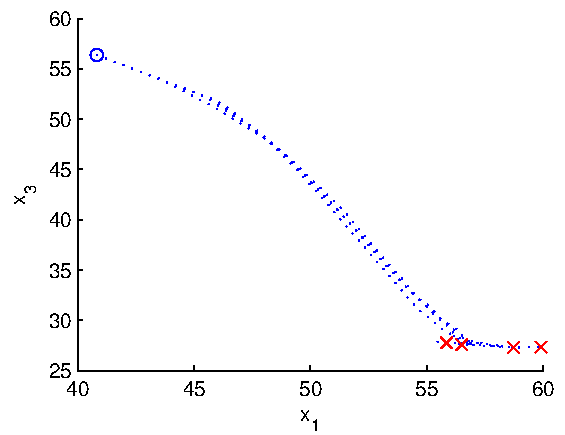
\includegraphics[width=0.45\columnwidth]{drone_example_rm.pdf}}
\subfloat[]{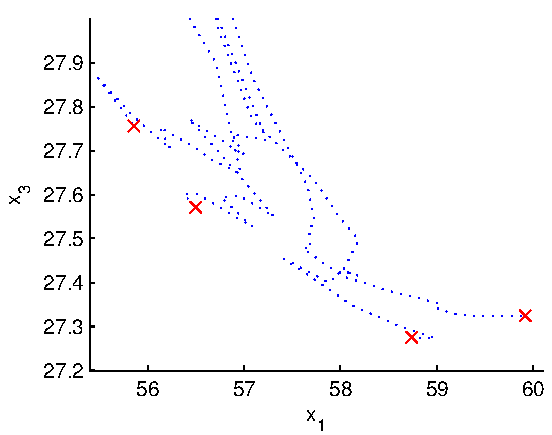
\includegraphics[width=0.45\columnwidth]{drone_example_rm_zoom.pdf}}
\caption{Four particle trajectories simulated from the same starting point using $\lgexpsf=0.3$, as used in the resample-move proposal stage. The second panel shows a close-up of the final states. This example uses the terrain tracking model from section~\ref{sec:numsim:tracking}, showing one horizontal and the vertical state component. Prior states are shown with circles and posterior states with crosses.}
\label{fig:drone_rm_example}
\end{figure}



\section{Algorithm Summary and Comparisons with Existing Work}

The distinguishing novel components of the PPPF are the incremental state and weight update formulas for advancing the particles through pseudo-time. Algorithm~\ref{alg:pppf} summarises the PPPF.

\begin{algorithm}
\begin{algorithmic}[1]
  \FOR{$\ti=1,2,\dots$}
    \FOR{$i=1,\dots,N_F$}
      \IF{$\ti>1$}% and $\ess{\ti-1}$ less than threshold}
        \STATE Select an ancestor, $a_i=j$, with probability $\npw{\ti-1}\pss{a_i}$
      \ENDIF
      \STATE Initialise pseudo-time, $\pt=0$.
      \STATE Initialise state by sampling from the transition/prior density, $\ls{\ti,0}\pss{i} \sim \transden(\ls{\ti} | \ls{\ti-1}\pss{\anc{\ti}{i}})$ or $\ls{\ti,0}\pss{i} \sim \priorden(\ls{\ti})$.
      \STATE Initialise weight, $\pw{\ti,0}\pss{i} = 1$.
      \WHILE{$\pt<1$}
        \STATE Increment pseudo-time, $\pt \leftarrow \pt+\dpt$, using a fixed or adaptive method.
        \STATE Update state $\ls{\ti,\pt}\pss{i}$ using \eqref{eq:state_update}, and an appropriate Gaussian approximation.
        \STATE Update weight $\pw{\ti,\pt}\pss{i}$ using \eqref{eq:PPPF_deterministic_weight_update} or \eqref{eq:PPPF_stochastic_weight_update}.
      \ENDWHILE
      \STATE Finalise, $\ls{\ti}\pss{i} = \ls{\ti,1}\pss{i}$, $\pw{\ti}\pss{i} = \pw{\ti,1}\pss{i}$.
    \ENDFOR
    \STATE Normalise weights, $\npw{\ti} = \pw{\ti}\pss{i} / \sum_j \pw{\ti}\pss{j}$ .
  \ENDFOR
\end{algorithmic}
\caption{Progressive Proposal Particle Filter}
\label{alg:pppf}
\end{algorithm}

The progressive proposal method shares a number of features with existing algorithms. Here we highlight some of the similarities and differences.

The concept of introducing intermediate distributions between the predictive and filtering densities has been employed in numerous ways, under the names ``annealing'' \citep{Neal2001,Deutscher2000,Gall2007}, ``tempering'' \citep{DelMoral2006}, ``bridging distributions'' \citep{Godsill2001b} and ``progressive corrections'' \citep{Oudjane2000}. These all use a discrete set of intermediate times, and do not consider the continuous evolution of the states. Furthermore they rely on importance sampling, Metropolis-Hastings and kernel sampling, all stochastic mechanisms, to advance between these pseudo-times. None of them include a deterministic component for updating the state. Moreover, these methods all rely on moving the particles through pseudo-time on the same fixed grid, and make use of intermediate resampling and interaction steps. The idea of moving particles independently with adaptive step sizes is new.

Another family of algorithms, the ``particle flow'' and ``optimal transport'' particle filters of \citep{Daum2008,Daum2011d,Reich2011,Reich2012a}, do allow continuous evolution of the particles over pseudo-time. However, these algorithms use the sequence from the predictive to filtering density to guide the particle motion, rather than that from the transition density to the OID. If this could be achieved analytically then the particles would be always equally weighted, independent and perfectly distributed according to the posterior. However, in general it becomes necessary to make approximations, either functional or numerical, of the predictive density, the effects of which can be unpredictable and difficult to quantify. Furthermore, the convergence properties of an ordinary particle filter are lost, since these approximations are not accounted for through the use of a particle weight. In contrast, the particles of the PPPF are moved approximately according to the OID sequence, and their resulting distribution is defined to be the importance distribution for an importance sampling step. Hence the approximations are accounted for in the particle weights.



\section{Some Extensions to the PPPF}

\subsection{Progressive Proposals for a Subset of State Variables}\label{sec:pppf_for_state_subset}

Some latent state variables may not be amenable to using a progressive proposal, in particular discrete variables such as indicators. If the model has the following factorisable form,
%
\begin{IEEEeqnarray}{rCl}
 \els{\ti} & \sim & \transden_{\els{}}(\els{\ti} | \els{\ti-1}, \ls{\ti-1}) \nonumber \\
 \ls{\ti} & \sim & \transden_{\ls{}}(\ls{\ti} | \els{\ti}, \els{\ti-1}, \ls{\ti-1}) \nonumber \\
 \ob{\ti} & \sim & \obsden(\ob{\ti} | \ls{\ti}, \els{\ti}) \nonumber      ,
\end{IEEEeqnarray}
%
where $\els{\ti}$ is discrete (or otherwise problematic), then a progressive proposal may be used for inference of $\ls{\ti}$ only, while $\els{\ti}$ is sampled from an ordinary importance distribution at pseudo-time $0$.



\subsection{Scale Mixtures of Normals}

Approximating a general density function by a Gaussian such as with \eqref{eq:gaussianise_transden} or \eqref{eq:gaussianise_transden} can be crude, and often requires some heuristic adjustments to achieve good performance of the PPPF. A different method may be used for densities (either transition or observation) which may be represented as scale mixtures of normals.

A scale mixture of normals density may be written in the following form,
%
\begin{IEEEeqnarray}{rCl}
 \den(z) & = & \int \normal{z}{m}{\frac{1}{\mix{}}P} \den(\mix{}) d\mix{}     .
\end{IEEEeqnarray}
%
For example, if $\den(\mix{})$ is a chi-squared distribution (with $\dof$ degrees of freedom), then $\den(z)$ is a student-t distribution (also with $\dof$ degrees of freedom). With $1$ degree of freedom, this becomes a Cauchy distribution. Stable distributions may also be represented \citep{West1987,Godsill1999}.

If the target distribution is extended to include the auxiliary mixing variable $\mix{}$, then the model factorisation method outlined in section~\ref{sec:pppf_for_state_subset} may be used. The mixing variable is sampled from an importance density at $\pt=0$ and kept fixed throughout the progressive proposal. However, we can do better than this, by allowing the value of the mixing variable to change each time we make a new Gaussian approximation, and then remaining constant until the next update. It would be even more desirable to allow $\mix{\pt}$ to evolve continuously, but this does not lead to tractable update formulas.

Define a new target density sequence,
%
\begin{IEEEeqnarray}{rCl}
 \augfiltden{\pt}(\ls{1:\ti-1}, \ls{\pt}, \mix{\pt}) & = & \frac{ \obsden(\ob{\ti} | \ls{\pt}, \mix{\pt})^{\pt} \transden(\ls{\pt} | \ls{\ti-1}, \mix{\pt}) \den(\mix{\pt}) \den(\ls{1:\ti-1}|\ob{1:\ti-1}) }{ \augfiltnorm{\pt} } \label{eq:SMiN_filtering_sequence}      .
\end{IEEEeqnarray}
%
Starting at $\pt_0$, a new value $\mix{\pt_1}$ is first sampled for the interval $(\pt_0,\pt_1]$ from an importance density $\impden{\pt}(\mix{\pt})$, after which the state update is carried out as before, using \eqref{eq:state_update} (and an appropriate Gaussian approximation if required). The weight update formula with this modification becomes,
%
\begin{IEEEeqnarray}{rCl}
 \pw{\pt_1} & \propto & \pw{\pt_0} \times \frac{ \obsden(\ob{\ti} | \ls{\pt_1}, \mix{\pt_1})^{\pt_1} \transden(\ls{\pt_1} | \ls{\ti-1}, \mix{\pt_1}) \den(\mix{\pt_1}) }{ \obsden(\ob{\ti} | \ls{\pt_0}, \mix{\pt_0})^{\pt_0} \transden(\ls{\pt_0} | \ls{\ti-1}, \mix{\pt_0}) \den(\mix{\pt_0}) } \times \frac{\mathcal{N}(\ls{\pt_0}|\lgoimnapprox{\pt_0}{\ls{\pt_0}},\lgoivrapprox{\pt_0}{\ls{\pt_0}}) \impden{\pt_0}(\mix{\pt_0})} {\mathcal{N}(\ls{\pt_1}|\lgoimnapprox{\pt_1}{\ls{\pt_0}},\lgoivrapprox{\pt_1}{\ls{\pt_0}}) \impden{\pt_1}(\mix{\pt_1})} \nonumber       .
\end{IEEEeqnarray}

The simplest choice for $\impden{\pt}(\mix{\pt})$ is to use the prior $\den(\mix{\pt})$. This is very simple to implement, simplifies the weight formula, and has been shown to be effective in simulations. In addition, it can be used with stable distributions when the density function cannot be analytically evaluated. The optimal choice is to use the marginal conditional posterior,
%
\begin{IEEEeqnarray}{rCl}
 \impden{\pt}(\mix{\pt}) & \propto & \int \obsden(\ob{\ti} | \ls{\pt}, \mix{\pt})^{\pt} \transden(\ls{\pt} | \ls{\ti-1}, \mix{\pt}) \den(\mix{\pt}) d\ls{\pt} \nonumber      .
\end{IEEEeqnarray}
%
If the models are linear and Gaussian conditional on $\mix{\pt}$ then this may be sampled from using rejection sampling. Otherwise, it will be intractable.

The effect of sampling the mixing variable $\mix{\pt}$ is that for each step through pseudo-time, the state is updated according to a different conditionally-Gaussian model. Intuitively, this ``blend'' gives us a better approximation of the update corresponding to the true density. The larger the variance of $\den(\mix{\pt})$, the less effective this is likely to be.



\section{Simulations}

Numerical testing using simulated data is presented to demonstrate the efficacy of the PPPF. The aim in developing the progressive proposal method is to provide a more efficient particle filter for challenging nonlinear models. In such cases, simple Gaussian approximations often work poorly, because the posterior filtering distributions of such models can assume complex and irregular shapes. Unfortunately, this effect also makes the assessment of particle filter performance a serious challenge. Statistics such as root-mean-square error (RMSE) and normalised estimation error squared (NEES), based on only the first two moments of the distribution, may be misleading. See figure~\ref{fig:rmse_fail}, for example.
%
\begin{figure}
\centering
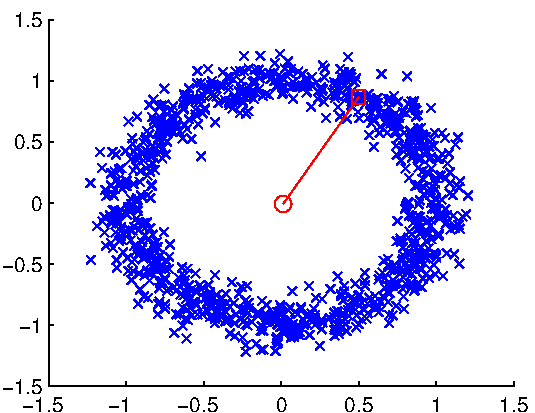
\includegraphics[width=0.7\columnwidth]{rmse_fail.pdf}
\caption{An illustration of how RMSE can be a misleading performance measure. A large number of samples (crosses) are drawn from the same distribution as the true value (square). The resulting sample mean (circle) is a very poor estimate of the true value, and the RMSE is large.}
\label{fig:rmse_fail}
\end{figure}

Our primary indicator of performance will be the average effective sample size, measured before resampling. RMSE values are also included but they should be treated with caution. All comparisons are conducted by adjusting the number of filter particles such that the running times for the various algorithms are roughly equal.

The following particle filters (and their respective importance densities) are used for comparison with the PPPF:
\begin{itemize}
        \item A bootstrap filter (BF), using the transition density.
        \item An extended particle filter (EPF), using a Gaussian density chosen by linearisation about the predictive mean, in the style of an extended Kalman filter.
        \item An unscented particle filter (UPF), using a Gaussian density chosen using the unscented transform, in the style of an unscented Kalman filter.
        \item An Laplacian approximation particle filter (LAPF), using a Gaussian density chosen by truncation of the Taylor series of the log of the unnormalised OID around a local maximum \citep{Doucet2000a}. Gradient ascent is used to locate the maximum.
\end{itemize}
%
Annealed particle filters are not included in the comparisons since the inter-dependence introduced between particles means that fair comparisons cannot be made using ESS.



\subsection{A Illustrative Problem}

\subsubsection{The Model}

The PPPF was tested on a modified form of the model used by \citet{Mihaylova2011}, which is a multivariate extension of the nonlinear benchmark model of \citep{Kitagawa1991}. The transition and observation functions are,
%
\begin{IEEEeqnarray}{rCl}
 \transfun(\ls{\ti-1}) & = & \half \ls{\ti-1} + 25 \frac{ \sum_d \ls{\ti-1,d} }{ 1 + \left(\sum_d \ls{\ti-1,d}\right)^2 } + 8 \cos(1.2 \ti) \nonumber \\
 \obsfun(\ls{\ti})_d   & = & \alpha \left( \ls{\ti,2d-1}^2 + \ls{\ti,2d}^2 \right) \nonumber      ,
\end{IEEEeqnarray}
%
where $\ls{\ti,d}$ and $\obsfun(\ls{\ti})_d$ are the $d$th components of the state vector and observation function respectively. A $10$-dimensional state and a $5$-dimensional observation were used. The transition and observation densities are Gaussian with $\lgmtv = 100 \times I$ and $\lgmov = I$.

This model is particularly challenging because the observations give us information only about the magnitudes of a set of sub-vectors of the state. Information about the corresponding bearing is only available via the transition model. Consequently, the region of high posterior probability corresponds to a ``thin'' section of the space bounding a hyper-sphere. A Gaussian density is a very poor approximation of this region. (See figure~\ref{fig:nlng_example_frame}.)

\subsubsection{Algorithms and Results}

Particle filters using extended or unscented Kalman-type importance densities fail immediately on this model; all the particles suffer numerical underflow of their weight due to states being sampled only in highly improbable regions. Tests were conducted on a BF, LAPF, and a deterministic PPPF (i.e. with $\lgexpsf=0)$. The PPPF employed the adaptive step size method, and typically required in the region of $10$ to $20$ state updates at each time step. Figure~\ref{fig:nlng_example_frame} shows the motion of the particles from the PPPF on a typical frame, and the awkward shape of the posterior mode. Table~\ref{tab:nlng_results} shows the average ESSs and RMSEs for each algorithm over 100 simulated data sets, each of 100 time steps.
%
\begin{table}
\centering
\begin{tabular}{l||c|c|c}
Algorithm                                & $N_F$ & ESS  & RMSE \\
\hline
Bootstrap                                & 18500 &  1.7 & 43.6 \\
Laplacian Approximation Proposal         &    70 &  1.7 & 42.8 \\
Deterministic Progressive Proposal       &   540 & 81.1 & 32.6 \\
\end{tabular}
\caption{Algorithm performance results on the multivariate benchmark model.}
\label{tab:nlng_results}
\end{table}
%
\begin{figure}
\centering
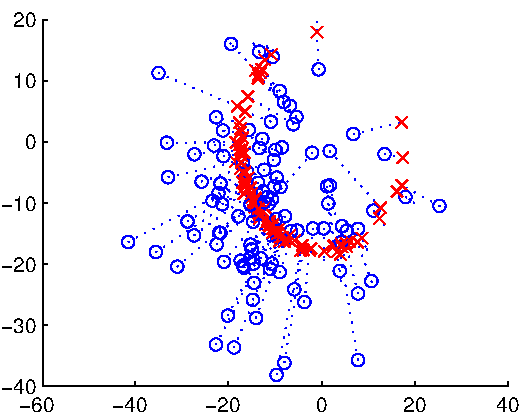
\includegraphics[width=0.7\columnwidth]{nlng_example_frame_deter.pdf}
\caption{An example of the PPPF particle motion running on the multivariate benchmark model, showing $2$ of the $10$ state dimensions. Prior states are shown with circles and posterior states with crosses.}
\label{fig:nlng_example_frame}
\end{figure}



\subsection{A Difficult Tracking Problem} \label{sec:numsim:tracking}

\subsubsection{The Model}

Next we consider tracking a small aircraft over a mapped landscape. Time of flight and Doppler measurements from a radio transmitter on the aircraft provide accurate measurements of range $\rng{\ti}$, and range rate $\rngrt{\ti}$, but only a low resolution measurement of bearing $\bng{\ti}$. In addition, accurate measurements are made of the height above the ground $\hei{\ti}$. The profile of the terrain (i.e. the height of the ground above a datum at each point) has been mapped.

At $\ti$, the latent state for our model is,
%
\begin{IEEEeqnarray}{rCl}
 \ls{\ti} & = & \begin{bmatrix} \pos{\ti} \\ \vel{\ti} \end{bmatrix} \nonumber      ,
\end{IEEEeqnarray}
%
where $\pos{\ti}$ and $\vel{\ti}$ are the $3$-dimensional position and velocity of the aircraft respectively, and the observation is,
%
\begin{IEEEeqnarray}{rCl}
 \ob{\ti} & = & \begin{bmatrix} \bng{\ti} \\ \rng{\ti} \\ \hei{\ti} \\ \rngrt{\ti} \end{bmatrix}       .
\end{IEEEeqnarray}
%
The observation function is described by the following equations,
%
\begin{IEEEeqnarray}{rCl}
 \bng{\ti}   & = & \arctan\left(\frac{\pos{\ti,1}}{\pos{\ti,2}}\right) \nonumber \\
 \rng{\ti}   & = & \sqrt{ \pos{\ti,1}^2 + \pos{\ti,3}^2 + \pos{\ti,3}^2 } \nonumber \\
 \hei{\ti}   & = & \pos{\ti,3} - \terrain( \pos{\ti,1}, \pos{\ti,2} ) \nonumber \\
 \rngrt{\ti} & = & \frac{ \pos{\ti}\cdot\vel{\ti} }{ \rng{\ti} } \nonumber      ,
\end{IEEEeqnarray}
%
where $\terrain( \pos{\ti,1}, \pos{\ti,2} )$ is the terrain height at the corresponding horizontal coordinates. The four measurements are independent and the respective variances are $\left(\frac{\pi}{9}\right)^2$, $0.1^2$, $0.1^2$, $0.1^2$.

Two linear transition models have been used, both based on a near-constant velocity model, one with a Gaussian density and one with a Student-t density with $\dof = 3$ degrees of freedom,
%
\begin{IEEEeqnarray}{rCl}
 \transden_1(\ls{\ti} | \ls{\ti-1}) & = & \normal{\ls{\ti}}{\lgmtm\ls{\ti-1}}{\lgmtv} \nonumber \\
 \transden_2(\ls{\ti} | \ls{\ti-1}) & = & \studentt{\ls{\ti}}{\lgmtm\ls{\ti-1}}{\lgmtv}{\dof} \nonumber      ,
\end{IEEEeqnarray}
%
\begin{IEEEeqnarray}{rCl}
 \lgmtm & = & \begin{bmatrix} I & I \\ 0 & I \end{bmatrix} \nonumber \\
 \lgmtv & = & 10 \begin{bmatrix} \frac{1}{3} I & \frac{1}{2} I \\ \frac{1}{2} I &\ I \end{bmatrix} \nonumber      .
\end{IEEEeqnarray}
%
For the simulations presented here, the terrain profile was modelled as a mixture of randomly-generated Gaussian blobs. An example is shown in figure~\ref{fig:drone_terrain_map}.

The accurate measurements of range, range rate and height constrain the region of high posterior probability to lie on a $3$ dimensional subspace, which can take some very irregular shapes (see figure~\ref{fig:drone_example_frame_deterministic}).
%
\begin{figure}
\centering
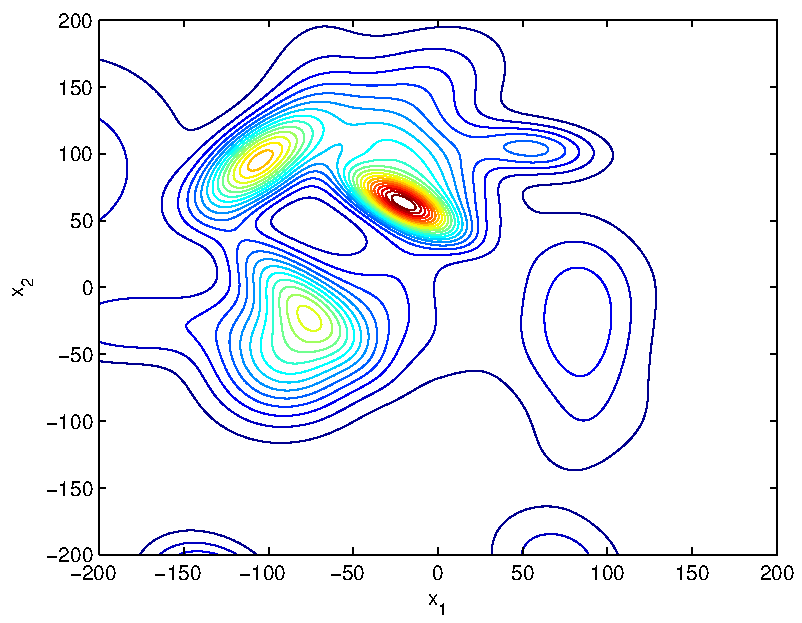
\includegraphics[width=0.7\columnwidth]{drone_terrain_map.pdf}
\caption{Contour plot of an example simulated terrain map.}
\label{fig:drone_terrain_map}
\end{figure}

\subsubsection{Algorithms and Results}

Particle filters using extended or unscented Kalman-type importance densities again did not perform well, with the EPF losing track immediately. Furthermore, the LAPF also performed particularly poorly as maximisation procedures struggle with the narrow mode. Tests were conducted on a BF, UPF, LAPF, and a deterministic PPPF (i.e. with $\lgexpsf=0)$. The PPPF employed the adaptive step size method, and uses in the region of $5$ to $10$ state updates at each time step. For the student-t transition density, the PPPF uses the scale mixture of normals method.

Figure~\ref{fig:drone_example_frame_deterministic} shows the motion of the particles from the deterministic PPPF on a typical frame, and the awkward shape of the posterior mode.
%
\begin{figure}
\centering
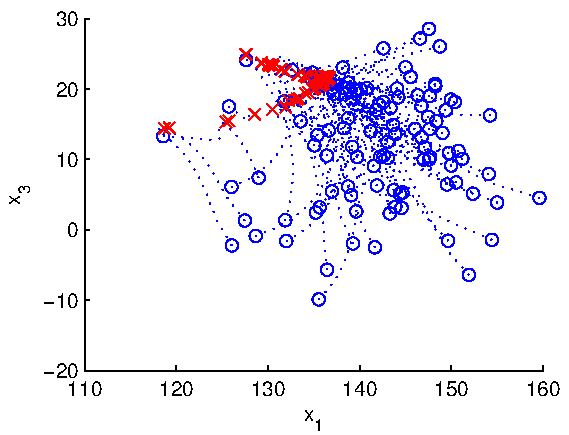
\includegraphics[width=0.7\columnwidth]{drone_example_frame_deter.pdf}
\caption{An example of the deterministic PPPF particle motion running on the terrain tracking model, showing one horizontal and the vertical state component. Prior states are shown with circles and posterior states with crosses.}
\label{fig:drone_example_frame_deterministic}
\end{figure}

A stochastic PPPF using resample-move was also tested. This obtained almost identical average RMSEs to the deterministic PPPF, but of course the resulting particle set has less inter-dependence between particles. Using $\lgexpsf=0.3$, roughly $25$--$50\%$ of the MH steps were accepted at each time step. Figure~\ref{fig:drone_example_frame_stochastic} shows the motion of the particles from the stochastic PPPF on a typical frame.
%
\begin{figure}
\centering
\subfloat[]{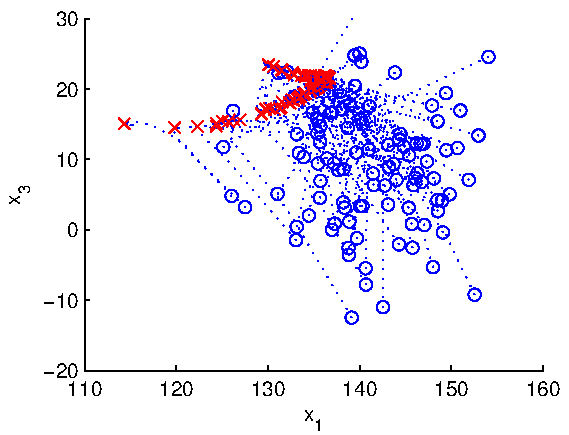
\includegraphics[width=0.45\columnwidth]{drone_example_frame.pdf}}
\subfloat[]{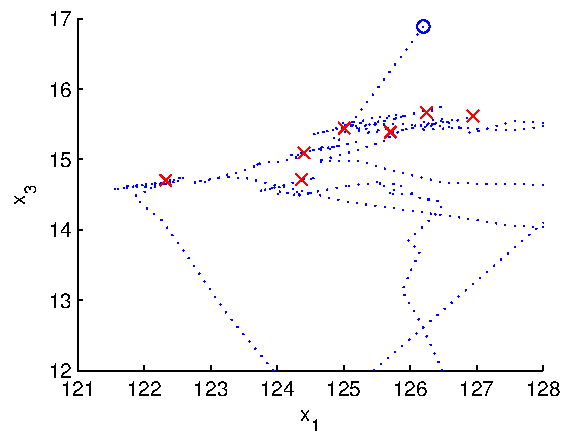
\includegraphics[width=0.45\columnwidth]{drone_example_frame_zoom.pdf}}
\caption{An example of the stochastic PPPF ($\lgexpsf=0.3$) particle motion running on the terrain tracking model, showing one horizontal and the vertical state component. Prior states are shown with circles and posterior states with crosses. The second panel is a close-up showing the stochastic motion of the particles.}
\label{fig:drone_example_frame_stochastic}
\end{figure}

Table~\ref{tab:drone_results_gaussian} shows the average ESSs and RMSEs for each algorithm over 100 simulated data sets, each of 100 time steps using the Gaussian transition density. The same is shown for the student-t transition density in table~\ref{tab:drone_results_studentt}.
%
\begin{table}
\centering
\begin{tabular}{l||c|c|c}
Algorithm                                & $N_F$ & ESS  & RMSE \\
\hline
Bootstrap                                &  6000 &  1.0 & 78.6 \\
Unscented Kalman Proposal                &   460 &  2.4 & 70.2 \\
Laplacian Approximation Proposal         &    10 &  3.1 & 62.9 \\
Deterministic Progressive Proposal       &   180 & 56.4 & 22.3 \\
\end{tabular}
\caption{Algorithm performance results on the terrain tracking model with Gaussian innovations.}
\label{tab:drone_results_gaussian}
\end{table}
%
\begin{table}
\centering
\begin{tabular}{l||c|c|c}
Algorithm                                & $N_F$ & ESS  & RMSE \\
\hline
Bootstrap                                &  6000 &  1.0 & 133.7 \\
Unscented Kalman Proposal                &   460 &  3.4 & 110.3 \\
Laplacian Approximation Proposal         &    10 &  2.9 & 105.1 \\
Deterministic Progressive Proposal       &   180 & 17.2 & 48.0 \\
\end{tabular}
\caption{Algorithm performance results on the terrain tracking model with student-t innovations.}
\label{tab:drone_results_studentt}
\end{table}

It was found that as $\dof$ is decreased, the performance of the progressive proposal particle filter deteriorated relative to the simpler algorithms, with the average ESS falling to around $6.0$ when $\dof=1$ (i.e. when the transition model has a Cauchy distribution). This is unsurprising, given that the scale of outliers increases as $\dof$ decreases.



\subsection{A Heartbeat Inference Problem}

\subsubsection{The Model}

As a final example, we consider the problem of detecting heartbeats in a vibration signal. Measurements from an accelerometer are first partitioned into segments believed to contain a heartbeat, and a particle filter is then used to infer its properties. The ($\ti$)th heartbeat is modelled parametrically as the product of a squared-exponential envelope with amplitude $\amp{\ti}$ and width $\wid{\ti}$, and a sine wave carrier with frequency $\freq{\ti}$ and relative phase $\pha{\ti}$. The time shift of the centre of the heartbeat within the measurement is $\del{\ti}$, and the sensor exhibits a D.C. bias $\bias{\ti}$ which varies slowly over time. The resulting observation function is highly nonlinear, with the ($d$)th component given by,
%
\begin{IEEEeqnarray}{rCl}
 \obsfun(\ls{\ti})_d & = & \amp{\ti} \exp\left\{ -\frac{ (T\,d - \del{\ti})^2 }{ 2\wid{\ti}^2 } \right\} \sin\left( \freq{\ti}(T\,d - \del{\ti}) + \pha{\ti} \right) + \bias{\ti} \nonumber      ,
\end{IEEEeqnarray}
%
where $T$ is the sampling period of the sensor. Each observation consists of $50$ time samples and the observation density is modelled as a Gaussian with a covariance matrix $0.2^2 I$. An example heartbeat simulated from this model is shown in figure~\ref{fig:sineha_example_beat}.
%
\begin{figure}
\centering
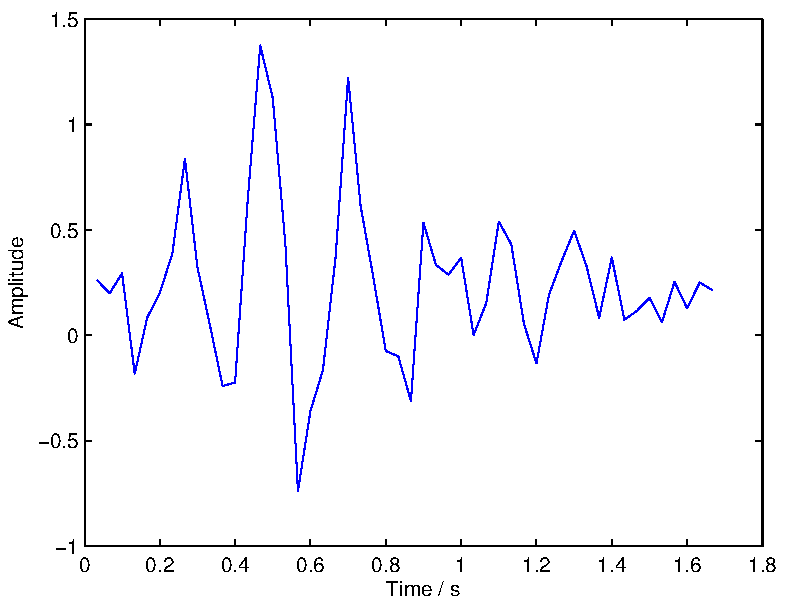
\includegraphics[width=0.7\columnwidth]{sineha_example_beat.pdf}
\caption{An example heartbeat simulated from the model.}
\label{fig:sineha_example_beat}
\end{figure}

The latent state is,
%
\begin{IEEEeqnarray}{rCl}
 \ls{\ti} & = & \begin{bmatrix} \amp{\ti} & \wid{\ti} & \del{\ti} & \freq{\ti} & \pha{\ti} & \bias{\ti} \end{bmatrix}^T      .
\end{IEEEeqnarray}
%
The transition density is factorised into independent terms, with $\freq{\ti}$, $\pha{\ti}$ and $\bias{\ti}$ evolving according to a Gaussian random walk, and $\wid{\ti}$ according to a geometric random walk (i.e. with a log-normal density), while $\del{\ti}$ and $\amp{\ti}$ are gamma distributed with no dependence on their past values.
%
%\begin{IEEEeqnarray}{rCl}
% \den(\amp{\ti} )                & = & \gammaden{\amp{\ti}-0.5}{10}{0.05} \nonumber \\
% \den(\wid{\ti} | \wid{\ti-1})   & = & \lognormal{\wid{\ti}}{}{} \nonumber \\
% \den(\del{\ti})                 & = &   \nonumber \\
% \den(\freq{\ti} | \freq{\ti-1}) & = &   \nonumber \\
% \den(\pha{\ti} | \pha{\ti-1})   & = &   \nonumber \\
% \den(\bias{\ti} | \bias{\ti-1}) & = &   \nonumber      ,
%\end{IEEEeqnarray}
%%
%where {\meta PARAMETERS}.

The likelihood is highly multi-modal, and hence so to is the filtering distribution.

\subsubsection{Algorithms and Results}

Particle filters using extended or unscented Kalman-type importance densities fail immediately on this model due to the highly multi-modal filtering distribution. Tests were conducted on a BF, LAPF, and a deterministic PPPF (i.e. with $\lgexpsf=0)$. For the PPPF, the transition density is approximated by a Gaussian using the method described in section~\ref{sec:non_gaussian_models}. The PPPF uses the adaptive step size method and made in the region of $5$ to $15$ state updates per time step, with the exception of a few particles which tended to ``get stuck'' and which were discarded after 50 steps.

Figure~\ref{fig:sineha_example_frame} shows the motion of the particles from the deterministic PPPF on a typical frame. Table~\ref{tab:sineha_results} shows the average ESSs and RMSEs for each algorithm over 100 simulated data sets, each of 100 time steps.
%
\begin{table}
\centering
\begin{tabular}{l||c|c|c}
Algorithm                                & $N_F$ & ESS  & RMSE \\
\hline
Bootstrap                                & 15000 &  7.6 &  2.0 \\
Laplacian Approximation Proposal         &   200 &  8.8 &  2.0 \\
Deterministic Progressive Proposal       &   800 & 72.8 &  1.4 \\
\end{tabular}
\caption{Algorithm performance results on the heartbeat inference model.}
\label{tab:sineha_results}
\end{table}
%
\begin{figure}
\centering
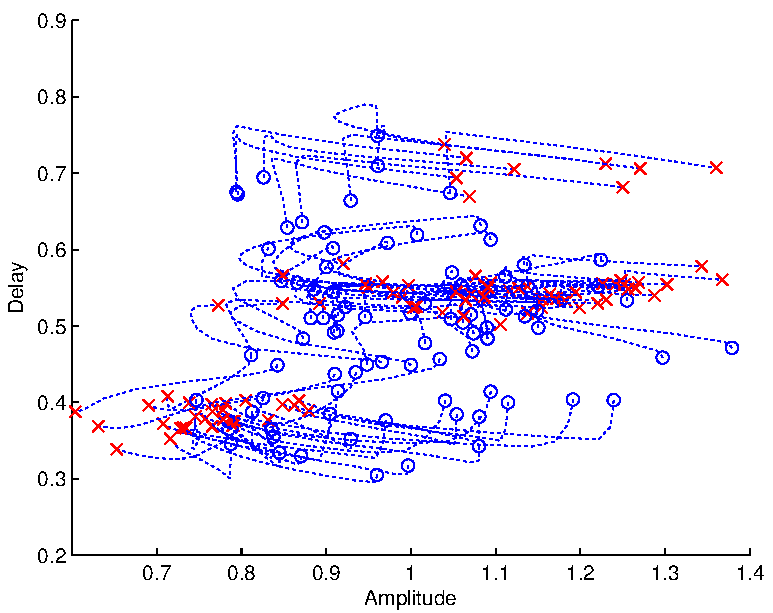
\includegraphics[width=0.7\columnwidth]{sineha_example_frame.pdf}
\caption{An example of the PPPF particle motion running on the heartbeat inference model, showing amplitude and delay state components. Prior states are shown with circles and posterior states with crosses.}
\label{fig:sineha_example_frame}
\end{figure}



\section{Summary and Conclusions}

We have detailed a new mechanism for conducting the update state in a particle filter, the progressive proposal method. This works by introducing the effect of the observation progressively and adjusting the particle state incrementally so as to achieve a better distribution.

The simulations presented in the previous section demonstrate that the progressive proposal procedure is capable of achieving better particle approximations (i.e. higher effective sample sizes) than simpler particle filters (which use a simple Gaussian importance density) on a class of challenging state space models. Furthermore, the particles thus generated are independent conditional on the resampled particle set from the preceding time step, a property not achieved by filters using annealing or resample-move.

The models for which the progressive proposal particle filter appears most effective are those with Gaussian transition and observation densities but highly nonlinear transition and observation functions. For this class, the performance improvement relative to the simpler algorithms with an equal processing time is very great. Moreover, the requisite Gaussian approximation is ``obvious'', simply a linearisation of the observation function, meaning that the algorithm requires almost no tuning (the tolerance for the adaptive step-size selection process is the only critical parameter).

With non-Gaussian model densities, the performance gains from the progressive proposal particle filter are more modest, when using either the scale mixture of normals method or Gaussian approximations formed by matching the gradient and Hessian of the optimal log-density. In addition, when more drastic approximations are required, a greater degree of algorithm tuning is required, such as limiting the variance of the approximation to prevent instability.

In general, there is no guarantee that the progressive proposal particle filter will outperform any other particle filter, not even a bootstrap filter. Indeed pathological examples may be constructed on which it will be inferior to the competition. However, the same may be said of all existing approximations to the optimal importance density. The choice of the right algorithm will often require a comparison on the particular application being studied.



\appendix

\section{Appropriate Dynamics Leading to a Standard Gaussian Stationary Distribution} \label{app:stationary_ou_process}

By using a Gaussian approximation, appropriate state update formulas may be derived by consideration of an underlying standard Gaussian variable,
%
\begin{IEEEeqnarray}{rCl}
 \ls{\pt} & = & \lgoimn{\pt} + \lgoivr{\pt}^{\half} \stdnorm{\pt} \nonumber \\ \\
 \stdnorm{\pt} & \sim & \normal{\stdnorm{\pt}}{0}{I} \nonumber      .
\end{IEEEeqnarray}

There is an infinitude of possible dynamical systems which maintain the correct marginal distribution. We narrow this down with the pragmatic approach that the system should be analytically integrable. Such is the case for a stationary Ornstein-Uhlenbeck process governed by,
%
\begin{IEEEeqnarray}{rCl}
 d\stdnorm{\pt} & = & - \oudrift{\pt} \stdnorm{\pt} d\pt + \oudiffuse{\pt} d\lginfbm{\pt} \nonumber      ,
\end{IEEEeqnarray}
%
subject to $\oudiffuse{\pt}\oudiffuse{\pt}^T = \oudrift{\pt}+\oudrift{\pt}^T$. The condition arises from writing the variance a short time in the future,
%
\begin{IEEEeqnarray}{rCl}
 \variance{}\left[\stdnorm{\pt+\dpt}\right] & = & \variance{}\left[ \stdnorm{\pt} - \oudrift{} \stdnorm{\pt} \dpt + \oudiffuse{} \delta\lginfbm{\pt} + \bigo{\dpt^2} \right] \nonumber \\
 & = & \variance{}\left[ \left(I-\dpt\oudrift{}\right) \stdnorm{\pt} \right] + \variance{}\left[ \oudiffuse{} \delta \lginfbm{\pt} \right] + \variance{}\left[ \bigo{\dpt^2} \right] \nonumber \\
 & = & I + \dpt\left[\oudiffuse{\pt}\oudiffuse{\pt}^T - \left(\oudrift{\pt}+\oudrift{\pt}^T\right)\right] + \bigo{\dpt^2} \nonumber      ,
\end{IEEEeqnarray}
%
and recalling that this variance must equal $I$.

Next consider the form of $\oudrift{\pt}$. In order to avoid arbitrary biases in a particular direction of $\stdnorm{\pt}$, this should be proportional to the identity matrix. Finally, since the increments $d\lginfbm{\pt}$ are independent and rotating does not affect their distribution, $\oudiffuse{\pt}$ may be made positive semidefinite without loss of generality, and hence must also be diagonal. Together, these conditions leave us with the following form for the stochastic differential equation (SDE),
%
\begin{IEEEeqnarray}{rCl}
 d\stdnorm{\pt} & = & -\half \lgexpsf \stdnorm{\pt} d\pt + \lgexpsf^{\half} d\lginfbm{\pt} \nonumber      .
\end{IEEEeqnarray}

Applying It\={o}'s lemma to the function $\exp\left\{\half\lgexpsf\pt\right\}\stdnorm{\pt}$, we find
%
\begin{IEEEeqnarray}{rCl}
 d\left[\exp\left\{\half\lgexpsf\pt\right\}\stdnorm{\pt}\right] & = & \half \lgexpsf \exp\left\{\half\lgexpsf\pt\right\}\stdnorm{\pt} d\pt + \exp\left\{\half\lgexpsf\pt\right\} d\stdnorm{\pt} \nonumber \\
 & = & \exp\left\{\half\lgexpsf\pt\right\} \left[ d\stdnorm{\pt} + \half \lgexpsf \stdnorm{\pt} d\pt \right] \nonumber \\
 & = & \lgexpsf^{\half} \exp\left\{\half\lgexpsf\pt\right\} d\lginfbm{\pt} \nonumber
\end{IEEEeqnarray}
%
Integrating leads to,
%
\begin{IEEEeqnarray}{rCl}
 \left[\exp\left\{\half\lgexpsf\pt\right\}\stdnorm{\pt}\right]_{\pt_0}^{\pt_1} & = & \int_{\pt_0}^{\pt_1} \lgexpsf^{\half} \exp\left\{\half\lgexpsf\pt\right\} d\lginfbm{\pt} \label{app-eq:stdnorm_stochastic_integral} \\
 \exp\left\{\half\lgexpsf\pt_1\right\} \stdnorm{\pt_1} - \exp\left\{\half\lgexpsf\pt_0\right\} \stdnorm{\pt_0} & = & \left[ \exp\left\{\lgexpsf\pt_1\right\} - \exp\left\{\lgexpsf\pt_0\right\} \right]^{\half} \stdnorm{\Delta} \nonumber     ,
\end{IEEEeqnarray}
%
where $\stdnorm{\Delta}$ is a new, standard Gaussian random variable, independent of $\stdnorm{\pt_0}$, and so,
%
\begin{IEEEeqnarray}{rCl}
 \stdnorm{\pt_1} & = & \exp\left\{ -\half \lgexpsf (\pt_1-\pt_0) \right\} \stdnorm{\pt_0} + \left[ 1 - \exp\left\{ - \lgexpsf (\pt_1-\pt_0) \right\} \right]^{\half} \stdnorm{\Delta} \nonumber       .
\end{IEEEeqnarray}

When considering error estimates for step size control, the following approximation of \ref{app-eq:stdnorm_stochastic_integral} for small intervals will also be useful,
%
\begin{IEEEeqnarray}{rCl}
 \int_{\pt_0}^{\pt_1} \lgexpsf^{\half} \exp\left\{\half\lgexpsf\pt\right\} d\lginfbm{\pt} & = & \exp\left\{\half\lgexpsf \pt_1 \right\} \left[ 1 - \exp\left\{ - \lgexpsf (\pt_1-\pt_0) \right\} \right]^{\half} \stdnorm{\Delta} \nonumber \\
 \lgexpsf^{\half} \exp\left\{\half\lgexpsf \pt_1 \right\} \int_{\pt_0}^{\pt_1} d\lginfbm{\pt} & \approx & \exp\left\{\half\lgexpsf \pt_1 \right\} \lgexpsf^{\half} (\pt_1-\pt_0)^{\half} \stdnorm{\Delta} \nonumber \\
 \int_{\pt_0}^{\pt_1} d\lginfbm{\pt} & \approx & (\pt_1-\pt_0)^{\half} \stdnorm{\Delta} \nonumber       .
\end{IEEEeqnarray}



\section{A Stochastic Differential Equation For State Evolution} \label{app:state_SDE}

For clarity, write $\lgoimn{\pt}$ instead of $\lgoimnapprox{\pt}{\pt_0}$ and $\lgoivr{\pt}$ instead of $\lgoivrapprox{\pt}{\pt_0}$ in this appendix.

The state $\ls{\pt}$ is a modelled as linear transformation of an underlying standard Gaussian random variable,
%
\begin{IEEEeqnarray}{rCl}
 \ls{\pt} & = & \lgoimn{\pt} + \lgoivr{\pt}^{\half} \stdnorm{\pt} \label{app-eq:gaussian_decomposition} \\
 \stdnorm{\pt} & \sim & \normal{\stdnorm{\pt}}{0}{I} \nonumber      .
\end{IEEEeqnarray}

This underlying variable is made to vary according to a stationary Ornstein-Uhlenbeck process,
%
\begin{IEEEeqnarray}{rCl}
 d\stdnorm{\pt} & = & -\half \lgexpsf \stdnorm{\pt} d\pt + \lgexpsf^{\half} d\lginfbm{\pt} \label{app-eq:standard_normal_SDE}      .
\end{IEEEeqnarray}

Differentiating \eqref{app-eq:gaussian_decomposition} using It\={o}'s Lemma and substituting \eqref{app-eq:standard_normal_SDE},
%
\begin{IEEEeqnarray}{rCl}
 d\ls{\pt} & = & \frac{\partial \lgoimn{\pt}}{\partial \pt} d\pt + \half \frac{\partial \lgoivr{\pt} }{\partial \pt} \lgoivr{\pt}^{-\half} \stdnorm{\pt} d\pt + \lgoivr{\pt}^{\half} d\stdnorm{\pt} \nonumber \\
 & = & \frac{\partial \lgoimn{\pt}}{\partial \pt} d\pt + \half \frac{\partial \lgoivr{\pt} }{\partial \pt} \lgoivr{\pt}^{-1} \left(\ls{\pt}-\lgoimn{\pt}\right) d\pt \nonumber \\
 &   & \qquad \qquad + \: \lgoivr{\pt}^{\half} \left[ -\half \lgexpsf \lgoivr{\pt}^{-\half} \left(\ls{\pt}-\lgoimn{\pt}\right) d\pt + \lgexpsf^{\half} d\lginfbm{\pt} \right] \nonumber \\
 & = & \left[ \frac{\partial \lgoimn{\pt}}{\partial \pt} + \half \left( \frac{\partial \lgoivr{\pt} }{\partial \pt} \lgoivr{\pt}^{-1} - \lgexpsf I \right) (\ls{\pt}-\lgoimn{\pt}) \right] d\pt + \lgexpsf^{\half} \lgoivr{\pt}^{\half} d\lginfbm{\pt}      .
\end{IEEEeqnarray}

%{\meta Cut this to another appendix, or elaborate further.}
%
%In the partially linear-Gaussian case, or when the Gaussian OID approximation takes the following form,
%%
%\begin{IEEEeqnarray}{rCl}
% \lgoivr{\pt} & = & \left[ \lgmtv^{-1} + \pt \lgmom^T \lgmov^{-1} \lgmom \right]^{-1} \nonumber \\
% \lgoimn{\pt}    & = & \lgoivr{\pt} \left[ \lgmtv^{-1} \transfun(\ls{\ti-1}) + \pt \lgmom^T \lgmov^{-1} \ob{\ti} \right] \nonumber     ,
%\end{IEEEeqnarray}
%%
%then
%%
%\begin{IEEEeqnarray}{rCl}
% \frac{\partial \lgoivr{\pt} }{\partial \pt} & = & -\lgoivr{\pt} \lgmom^T \lgmov^{-1} \lgmom \lgoivr{\pt} \nonumber \\
% \frac{\partial \lgoimn{\pt}}{\partial \pt} & = & \lgoivr{\pt} \lgmom^T \lgmov^{-1}(\ob{\ti}-\lgmom\lgoimn{\pt}) \nonumber       ,
%\end{IEEEeqnarray}
%%
%and the state evolution stochastic differential equation becomes,
%%
%\begin{IEEEeqnarray}{rCl}
% d\ls{\pt} & = & \left[ \lgoivr{\pt} \lgmom^T \lgmov^{-1} \left( (\ob{\ti}-\lgmom\lgoimn{\pt}) - \half \lgmom (\ls{\pt}-\lgoimn{\pt}) \right) - \half \lgexpsf (\ls{\pt}-\lgoimn{\pt}) \right] d\pt + \lgexpsf^{\half} \lgoivr{\pt}^{\half} d\lginfbm{\pt} \nonumber       .
%\end{IEEEeqnarray}

\section{Governing Equation for Optimal Particle Transport} \label{app:optimal_flow_governing_eq}

This exposition is based closely on that of \cite{Daum2008}, but we consider moving each particle according to its OID sequence rather than the filtering sequence. We omit the time subscripts, particle superscripts and the dependence on $\ls{\ti-1}$ for clarity. Define the following,
%
\begin{IEEEeqnarray}{rCl}
 \logtrans(\ls{}) & = & \log\left(\transden(\ls{}|\ls{\ti-1})\right) \nonumber \\
 \logobs(\ls{}) & = & \log\left(\obsden(\ob{\ti}|\ls{})\right) \nonumber \\
 \logoiden{\pt}(\ls{}) & = & \log\left( \oiden{\pt}(\ls{}) \right) \nonumber       .
\end{IEEEeqnarray}
%
The log-OID is therefore,
%
\begin{IEEEeqnarray}{rCl}
 \logoiden{\pt}(\ls{\pt}) & = & \logtrans(\ls{\pt}) + \pt \logobs(\ls{\pt}) - \log\left(\oinorm{\pt}\right) \nonumber     ,
\end{IEEEeqnarray}
%
and differentiating this,
%
\begin{IEEEeqnarray}{rCl}
 \pdv{\logoiden{\pt}}{\pt} & = & \logobs(\ls{\pt}) - \frac{d}{d\pt}\log\left(\oinorm{\pt}\right) \nonumber      .
\end{IEEEeqnarray}
%
Now since,
%
\begin{IEEEeqnarray}{rCl}
 \frac{d}{d\pt}\log\left(\oinorm{\pt}\right) & = & \frac{1}{\oinorm{\pt}} \frac{d\oinorm{\pt}}{d\pt} \nonumber \\
                                               & = & \frac{ \int \transden(\ls{}|\ls{\ti-1}) \obsden(\ob{\ti}|\ls{})^\pt \logobs(\ls{}) d\ls{} }{ \int \transden(\ls{}|\ls{\ti-1}) \obsden(\ob{\ti}|\ls{})^\pt d\ls{} } \nonumber \\
                                               & = & \int \oiden{\pt}(\ls{} | \ls{\ti-1}) \logobs(\ls{}) d\ls{} \nonumber \\
                                               & = & \expect{\oiden{\pt}}\left[ \logobs(\ls{}) \right] \nonumber     ,
\end{IEEEeqnarray}
%
this may be written as,
%
\begin{IEEEeqnarray}{rCl}
 \pdv{\logoiden{\pt}}{\pt} & = & \logobs(\ls{\pt}) - \expect{\oiden{\pt}}\left[ \logobs(\ls{}) \right] \label{app-eq:oid_logdensity}      .
\end{IEEEeqnarray}

The Fokker-Planck equation relates the flow of a particle with the evolution of the density for its position. For a particle moving according to,
%
\begin{IEEEeqnarray}{rCl}
 d\ls{\pt} & = & \flowdrift{\pt}(\ls{\pt}) d\pt + \flowdiffuse{\pt} d\flowbm{\pt} \nonumber     ,
\end{IEEEeqnarray}
%
Fokker-Planck then states,
%
\begin{IEEEeqnarray}{rCl}
 \pdv{\oiden{\pt}}{\pt} & = & - \nabla \cdot \left[ \flowdrift{\pt}(\ls{\pt}) \oiden{\pt}(\ls{\pt}) \right] + \nabla \cdot \left[ \flowcov{\pt} \nabla \oiden{\pt}(\ls{\pt}) \right] \nonumber \\
 & = & - \trace\left[ \pdv{}{\ls{\pt}}\left( \flowdrift{\pt}(\ls{\pt}) \oiden{\pt}(\ls{\pt}) \right) \right] + \trace\left[ \pdv{}{\ls{\pt}}\left( \flowcov{\pt} \pdv{\oiden{\pt}}{\ls{\pt}} \right) \right] \nonumber      ,
\end{IEEEeqnarray}
%
where,
%
\begin{IEEEeqnarray}{rCl}
 \flowcov{\pt} & = & \frac{1}{2} \flowdiffuse{\pt} \flowdiffuse{\pt}^T \nonumber      .
\end{IEEEeqnarray}

This may be recast using log-densities instead of densities using the following identities,
%
\begin{IEEEeqnarray}{rCl}
 \pdv{\logoiden{\pt}}{\pt} & = & \frac{ 1 }{ \oiden{\pt}(\ls{\pt}) } \pdv{\oiden{\pt}}{\pt} \nonumber \\
 \pdv{\logoiden{\pt}}{\ls{\pt}} & = & \frac{ 1 }{ \oiden{\pt}(\ls{\pt}) } \pdv{\oiden{\pt}}{\ls{\pt}} \nonumber \\
 \npdv{2}{\logoiden{\pt}}{\ls{\pt}} & = & \frac{ \oiden{\pt}(\ls{\pt}) \npdv{2}{\oiden{\pt}}{\ls{\pt}} - \pdv{\oiden{\pt}}{\ls{\pt}} \pdv{\oiden{\pt}}{\ls{\pt}}^T }{ \oiden{\pt}(\ls{\pt})^2 } \nonumber \\
 & = & \frac{ 1 }{ \oiden{\pt}(\ls{\pt}) } \npdv{2}{\oiden{\pt}}{\ls{\pt}} - \pdv{\logoiden{\pt}}{\ls{\pt}}\pdv{\logoiden{\pt}}{\ls{\pt}}^T \nonumber     ,
\end{IEEEeqnarray}
%
leading to,
%
\begin{IEEEeqnarray}{rCl}
 \pdv{\logoiden{\pt}}{\pt} & = & \frac{1}{\oiden{\pt}(\ls{\pt})} \left\{ - \trace\left[ \pdv{}{\ls{\pt}}\left( \flowdrift{\pt}(\ls{\pt}) \oiden{\pt}(\ls{\pt}) \right) \right] + \trace\left[ \pdv{}{\ls{\pt}}\left( \flowcov{\pt} \pdv{\oiden{\pt}}{\ls{\pt}} \right) \right] \right\} \nonumber \\
 & = & \frac{1}{\oiden{\pt}(\ls{\pt})} \left\{  -\trace\left[ \oiden{\pt}(\ls{\pt}) \pdv{\flowdrift{\pt}}{\ls{\pt}} + \flowdrift{\pt}(\ls{\pt})^T \pdv{\oiden{\pt}}{\ls{\pt}} \right] + \trace\left[ \flowcov{\pt} \npdv{2}{\oiden{\pt}}{\ls{\pt}} \right]  \right\} \nonumber \\
 & = & \frac{1}{\oiden{\pt}(\ls{\pt})} \Bigg\{  -\trace\left[ \oiden{\pt}(\ls{\pt}) \pdv{\flowdrift{\pt}}{\ls{\pt}} + \oiden{\pt}(\ls{\pt}) \flowdrift{\pt}(\ls{\pt})^T \pdv{\logoiden{\pt}}{\ls{\pt}} \right]  \nonumber \\
 & & \qquad + \:  \trace\left[ \flowcov{\pt} \oiden{\pt}(\ls{\pt}) \left( \npdv{2}{\logoiden{\pt}}{\ls{\pt}} + \pdv{\logoiden{\pt}}{\ls{\pt}} \pdv{\logoiden{\pt}}{\ls{\pt}}^T \right)\right]  \Bigg\} \nonumber \\
 & = & -\trace\left[ \pdv{\flowdrift{\pt}}{\ls{\pt}} \right] - \flowdrift{\pt}(\ls{\pt})^T \pdv{\logoiden{\pt}}{\ls{\pt}} + \trace\left[ \flowcov{\pt} \npdv{2}{\logoiden{\pt}}{\ls{\pt}} \right] + \pdv{\logoiden{\pt}}{\ls{\pt}}^T \flowcov{\pt} \pdv{\logoiden{\pt}}{\ls{\pt}} \label{app-eq:oid_log_fp}       .
\end{IEEEeqnarray}
%
Dividing through by $\oiden{\pt}$ in the first step requires that this density be nowhere vanishing. Combining the equations for the log-OID \eqref{app-eq:oid_logdensity} with the partial differential equation for the log-density evolution \eqref{app-eq:oid_log_fp}, the governing equation for the optimal particle dynamics is reached.



\section{Progressive Proposal Continuous Limit Using Linearisation} \label{app:continuous_limit_and_linearisation}

For nonlinear Gaussian models, the suitability of using linearisation to conduct the OID approximation updates rests on the fact that the mixed partial derivatives for the true density and the approximation are equal. For the true density, from \eqref{eq:oid_logdensity_time_derivative},
%
\begin{IEEEeqnarray}{rCl}
 \pdv{\logoiden{\pt}}{\pt} & = & \logobs(\ls{\pt}) - \expect{\oiden{\pt}}\left[ \logobs(\ls{}) \right] \nonumber      ,
\end{IEEEeqnarray}
%
with
%
\begin{IEEEeqnarray}{rCl}
 \logobs(\ls{}) & = & \log\left(\obsden(\ob{\ti}|\ls{})\right) \nonumber \\
 & = & -\half \log\left(\determ{2\pi\lgmov}\right) - \half\left[ \left(\ob{\ti}-\obsfun(\ls{\pt})\right)^T \lgmov^{-1} \left(\ob{\ti}-\obsfun(\ls{\pt})\right) \right] \nonumber      .
\end{IEEEeqnarray}
%
and so,
%
\begin{IEEEeqnarray}{rCl}
 \mpdv{\logoiden{\pt}}{\ls{\pt}}{\pt} & = & \pdv{\logobs}{\ls{\pt}} \nonumber \\
 & = & \pdv{\obsfun}{\ls{\pt}}^T \lgmov^{-1} \ob{\ti} - \pdv{\obsfun}{\ls{\pt}}^T \lgmov^{-1} \obsfun(\ls{\pt}) \nonumber \\
 & = & \lgmomapprox{\ls{\pt}}^T \lgmov^{-1} \left( \ob{\ti} - \obsfun(\ls{\pt}) \right) \nonumber       .
\end{IEEEeqnarray}

On the other hand, for the chosen dynamics of the particle state described by \eqref{eq:continuous_limit_state_SDE}, we can find this mixed partial derivative by differentiating \eqref{eq:oid_log_fp},
%
\begin{IEEEeqnarray}{rCl}
 \mpdv{\logoidenapprox{\pt}}{\ls{\pt}}{\pt} & = & \pdv{}{\ls{\pt}} \left\{ -\trace\left[ \pdv{\flowdrift{\pt}}{\ls{\pt}} \right] - \flowdrift{\pt}(\ls{\pt})^T \pdv{\logoidenapprox{\pt}}{\ls{\pt}} + \trace\left[ \flowcov{\pt} \npdv{2}{\logoidenapprox{\pt}}{\ls{\pt}} \right] + \pdv{\logoidenapprox{\pt}}{\ls{\pt}}^T \flowcov{\pt} \pdv{\logoidenapprox{\pt}}{\ls{\pt}} \right\} \nonumber      ,
\end{IEEEeqnarray}
%
where
%
\begin{IEEEeqnarray}{rCl}
 \flowdrift{\pt}(\ls{\pt}) & = & \ctlgoivrapprox{\pt} \lgmomapprox{\ls{\pt}}^T \lgmov^{-1} \left( \left(\ob{\ti} - \obsfun(\ls{\pt}) \right) + \half \lgmomapprox{\ls{\pt}} (\ls{\pt}-\ctlgoimnapprox{\pt}) \right) - \half \lgexpsf (\ls{\pt}-\ctlgoimnapprox{\pt}) \nonumber
\end{IEEEeqnarray}
\begin{IEEEeqnarray}{rCl}
 \flowcov{\pt} & = & \half \lgexpsf \ctlgoivrapprox{\pt} \nonumber
\end{IEEEeqnarray}
\begin{IEEEeqnarray}{rCl}
 \logoidenapprox{\pt} & = & -\half \log\left(\determ{2\pi\ctlgoivrapprox{\pt}}\right) - \half\left[ \left(\ls{\pt}-\ctlgoimnapprox{\pt}\right)^T \ctlgoivrapprox{\pt}^{-1} \left(\ls{\pt}-\ctlgoimnapprox{\pt}\right) \right] \nonumber \\
 \pdv{\logoidenapprox{\pt}}{\ls{\pt}} & = & - \ctlgoivrapprox{\pt}^{-1} \left(\ls{\pt}-\ctlgoimnapprox{\pt}\right) \nonumber \\
 \npdv{2}{\logoidenapprox{\pt}}{\ls{\pt}} & = & - \ctlgoivrapprox{\pt}^{-1}\nonumber      .
\end{IEEEeqnarray}
%
Substituting in these terms, we find simply that,
%
\begin{IEEEeqnarray}{rCl}
 \mpdv{\logoidenapprox{\pt}}{\ls{\pt}}{\pt} & = & \lgmomapprox{\ls{\pt}}^T \lgmov^{-1} \left( \ob{\ti} - \obsfun(\ls{\pt}) \right) \nonumber       .
\end{IEEEeqnarray}

By repeatedly differentiating by $\ls{\pt}$, we can similarly show that,
%
\begin{IEEEeqnarray}{rCl}
 \nmpdv{k+1}{k}{\logoidenapprox{\pt}}{\ls{\pt}}{\pt} & = &  \nmpdv{k+1}{k}{\logoiden{\pt}}{\ls{\pt}}{\pt} \nonumber       ,
\end{IEEEeqnarray}
%
as required.



\bibliographystyle{chicago}
\bibliography{D:/pb404/Dropbox/PhD/thesisbib}
%\bibliography{/home/pete/Dropbox/PhD/OTbib}

\end{document}
